\documentclass[implementacija.tex]{subfiles}
\usepackage{subfiles}
\documentclass[12pt,oneside]{memoir} 
\usepackage[latinica]{matfmaster}
\usepackage{caption}
\usepackage{subcaption}
\begin{document}

\subsection{Instalacija}
Instaliranje Android aplikacija na mobilne telefone je moguće na više načina. Najjednostavniji nacin je preuzimanje aplikacije iz \textit{Google Play} prodavnice. Ako aplikacija nije dostupna preko prodavnice, moze se instalirati preuzimanjem datoteke u formatu \textbf{APK} (eng. \textit{Android Package}). \textbf{APK}predstavlja format datoteka koji OS Android koristi za instaliranje i distribuciju aplikacija. Ova datoteka se kreira u \textit{build} direktorijumu projekta nakon što se u \textit{Android Studio}-u odabere opcija \textit{build}. Za aplikaciju \textit{Daljinski za digitalnu televiziju} instalaciona datoteka se može preuzeti na narednom linku: \hyperlink{https://drive.google.com/file/d/1gBlfRibn4jrFDe3TTBCsHUq9MDowEBty/view?usp=drive_link}{daljinski.apk}. Klikom na preuzetu datoteku, koja se može naći u direktorijumu gde se čuvaju preuzete datoteke, pokreće se instalacija aplikacije.

Za potrebe testiranja aplikacije tokom implementacije najčešće se koriste dva načina instaliranja. Za njih je potrebno omogućiti opcije programera (eng. \textit{developer options}) na mobilnom uređaju i da se uređaj poveže pomoću USB kabla sa računarom na kom se nalazi k\^{o}d. Prva mogućnost pokretanja je da se u \textit{Android Studio}-u pritisne dugme \textit{Run}. Druga opcija je da na računaru postoji instaliran \textbf{adb} (eng. \textit{Android Debug Bridge}) i u terminalu da se pokrene komanda \verb|adb install app-debug.apk|. 

\subsection{Pokretanje i korišćenje}

Nakon instalacije aplikacije prilikom prvog pokretanja prikazuje se ekran prikazan na slici \ref{fig:dozvola} koji obaveštava korisnika da je potrebno dozvoliti korišćenje mikrofona. Nakon toga se prikazuje sistemsko obaveštenje o traženju dozvole sa opcijama da korisnik da dopuštenje ili ga odbije. Ovo obaveštenje može se videti na slici \ref{fig:sistemsko_obavestenje}. Ukoliko se ne da dopuštenje moguće je dati ga naknadno u podešavanjima telefona. U slučaju da ovo nije prvo pokretanje aplikacije ova dva obaveštenja neće biti prikazana.
Aplikacija započinje pretragu uređaja kao na slici \ref{fig:pretraga}. Kako je aplikacija napravljena u saradnji sa jednim stranim klijentom prikazaće se samo uređaji koji imaju instaliranu njihovu aplikaciju, a nalaze se na istoj mreži. Pretraga je ograničena na 15 sekundi. Nakon isteka vremena ukoliko se ne pronađe nijedan uređaj korisnik dobija adekvatno obaveštenje sa izborom da li da se zatvori aplikacija ili ponovo pokuša traženje. Ovo je prikazano na slici \ref{fig:nema_uredjaja}. 
Svi uređaji koji su pronađeni se ispisuju na ekranu kao na slici \ref{fig:pronadjeni_uredjaji} i moguće je kliknuti na bilo koji od njih. Pritiskom na naziv odgovarajućeg uređaja iskazuje se želja da bude izvršeno uparivanje sa tim uređajem. Na uređaju sa kojim se pokušava uparivanje se prikazuje četvorocifren broj kao na slici \ref{fig:kod_na_stb}. Polje za unos tog broja se prikazuje u aplikaciji kao na slici \ref{fig:polje_za_kod}. Nakon uspešnog unosa prikazaog na slici \ref{fig:kod_na_mobilnom} uređaji se uparuju, a uspešno uparivanje potvrđuje i prikaz daljinskog upravljača. Podržane funkcionalnosti su prikazane na slici  \ref{fig:opis_komandi}.

% ----------------------------------------------------
% \begin{figure}[h!]
% \centering
%     \begin{subfigure}
%   \centering
%   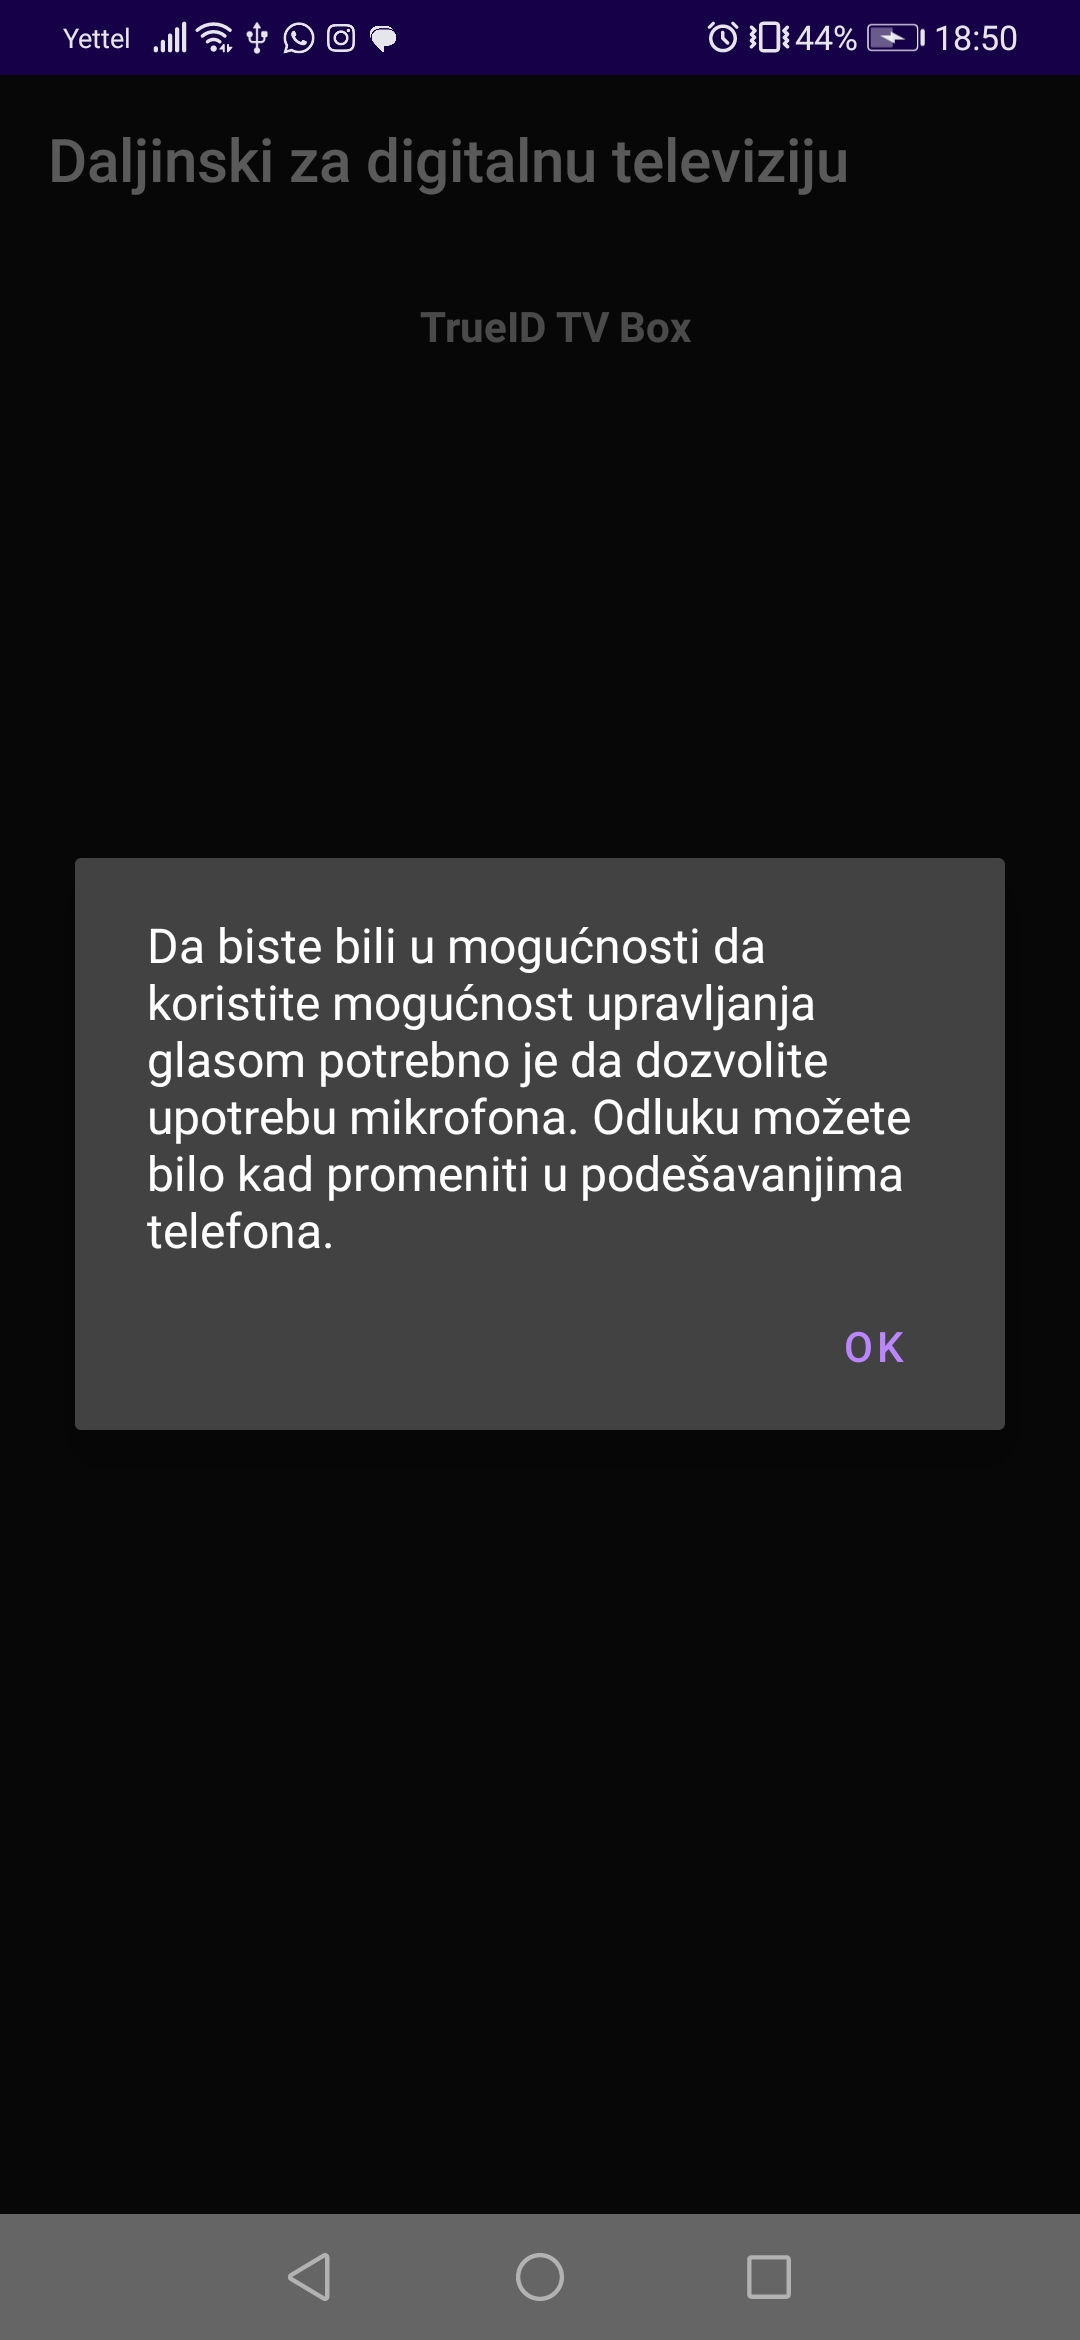
\includegraphics[width=9cm,height=9cm,keepaspectratio]{Implementacija/snimci_ekrana/1_obavestenje_za_dozvolu.jpg}
%   \caption{A obaveštenje o traženju dozvole}
%     \label{fig:dozvola}
%     \end{subfigure}%
%     \begin{subfigure}
%    \centering
%   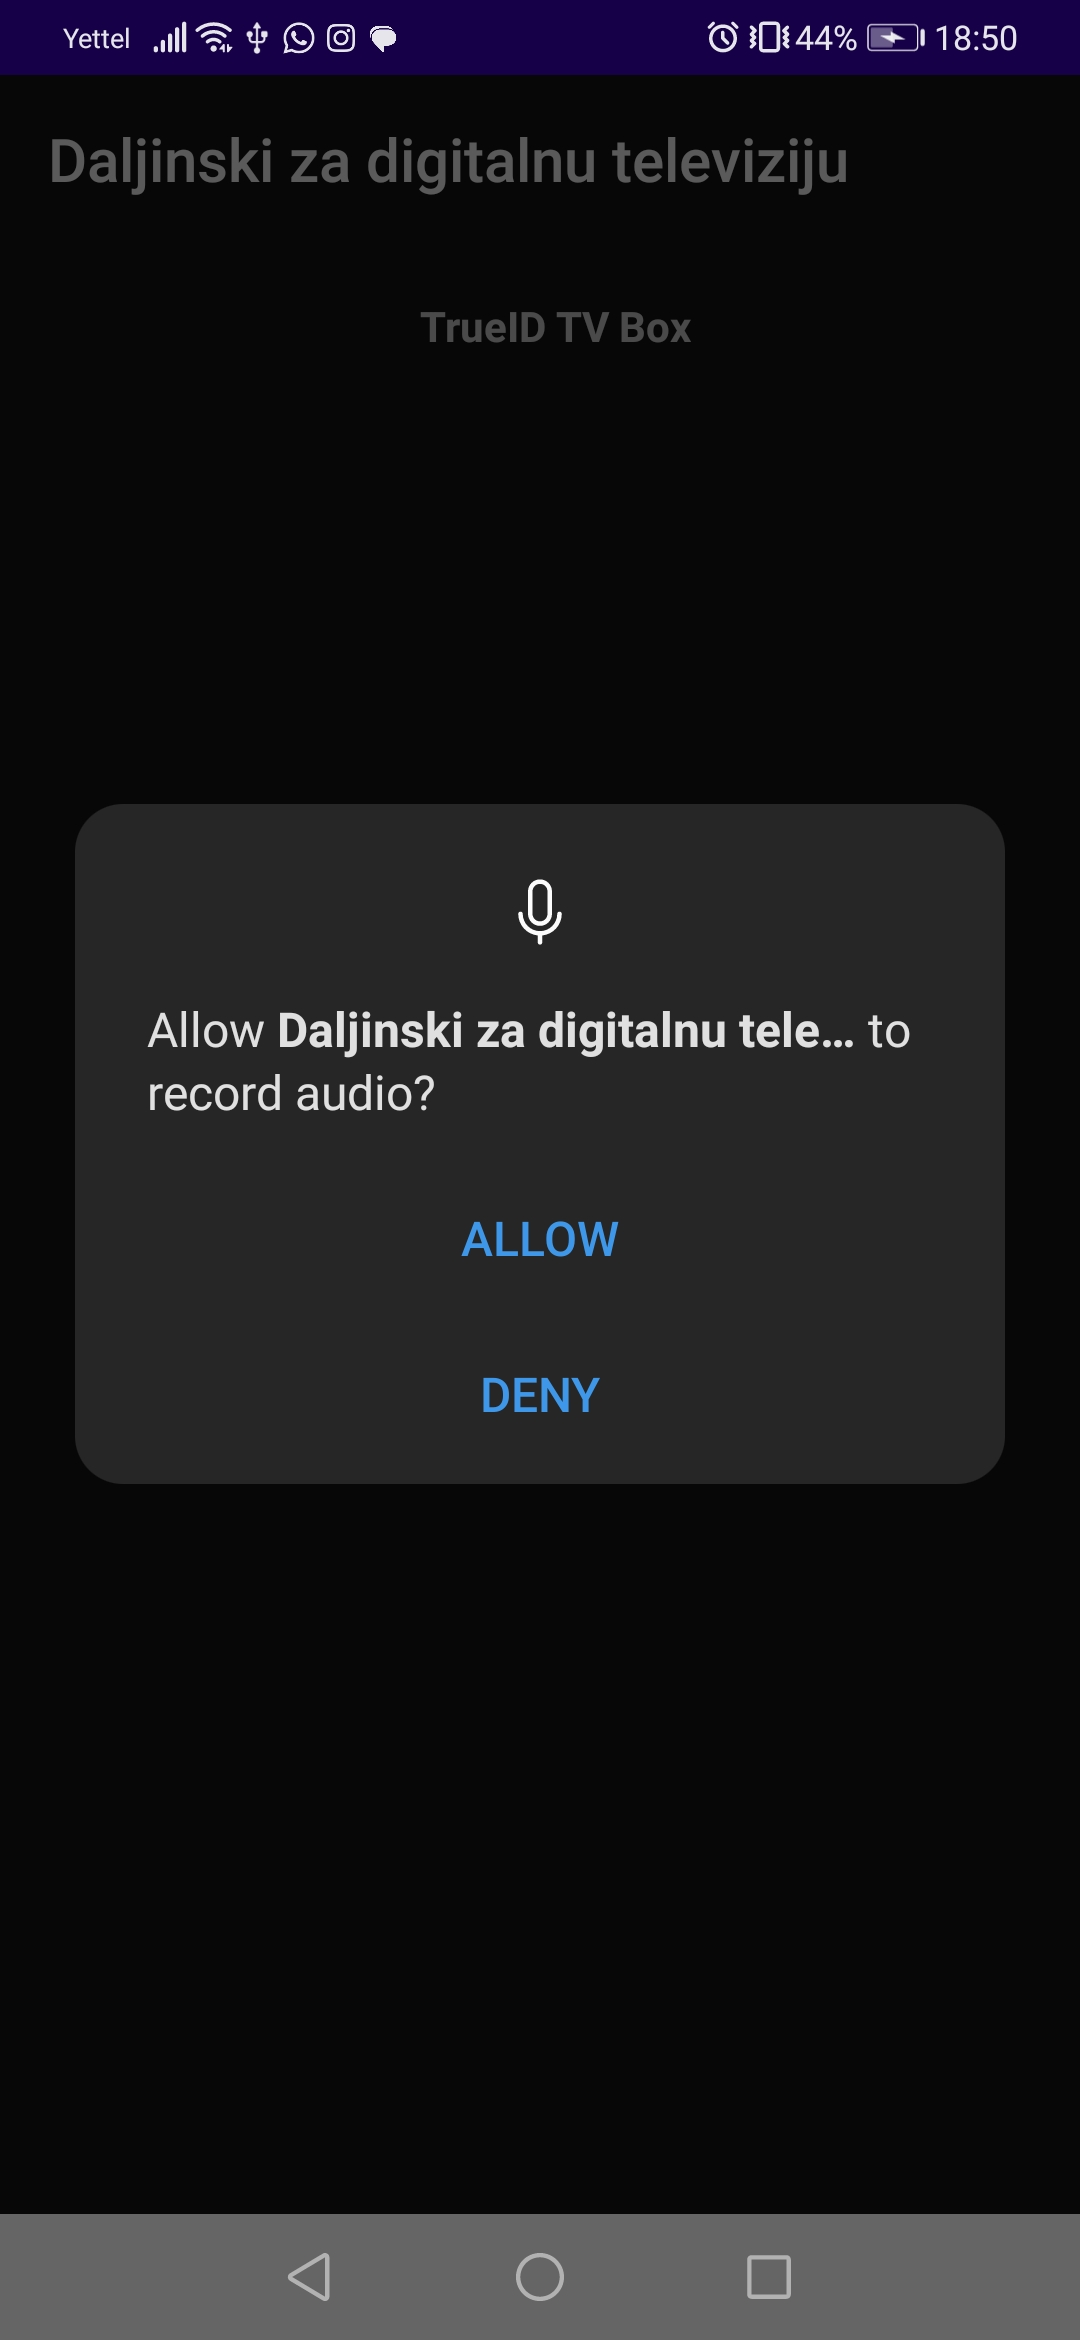
\includegraphics[width=9cm,height=9cm,keepaspectratio]{Implementacija/snimci_ekrana/2_sistemska_dozvola.jpg}
%   \caption{B prikaz sistemskog obaveštenja}
%     \label{fig:sistemsko_obavestenje}
%     \end{subfigure}
% \caption{Snimak ekrana}
% \label{fig:pocetni_ekrani}
% \end{figure}

\begin{figure}[h!]
\centering
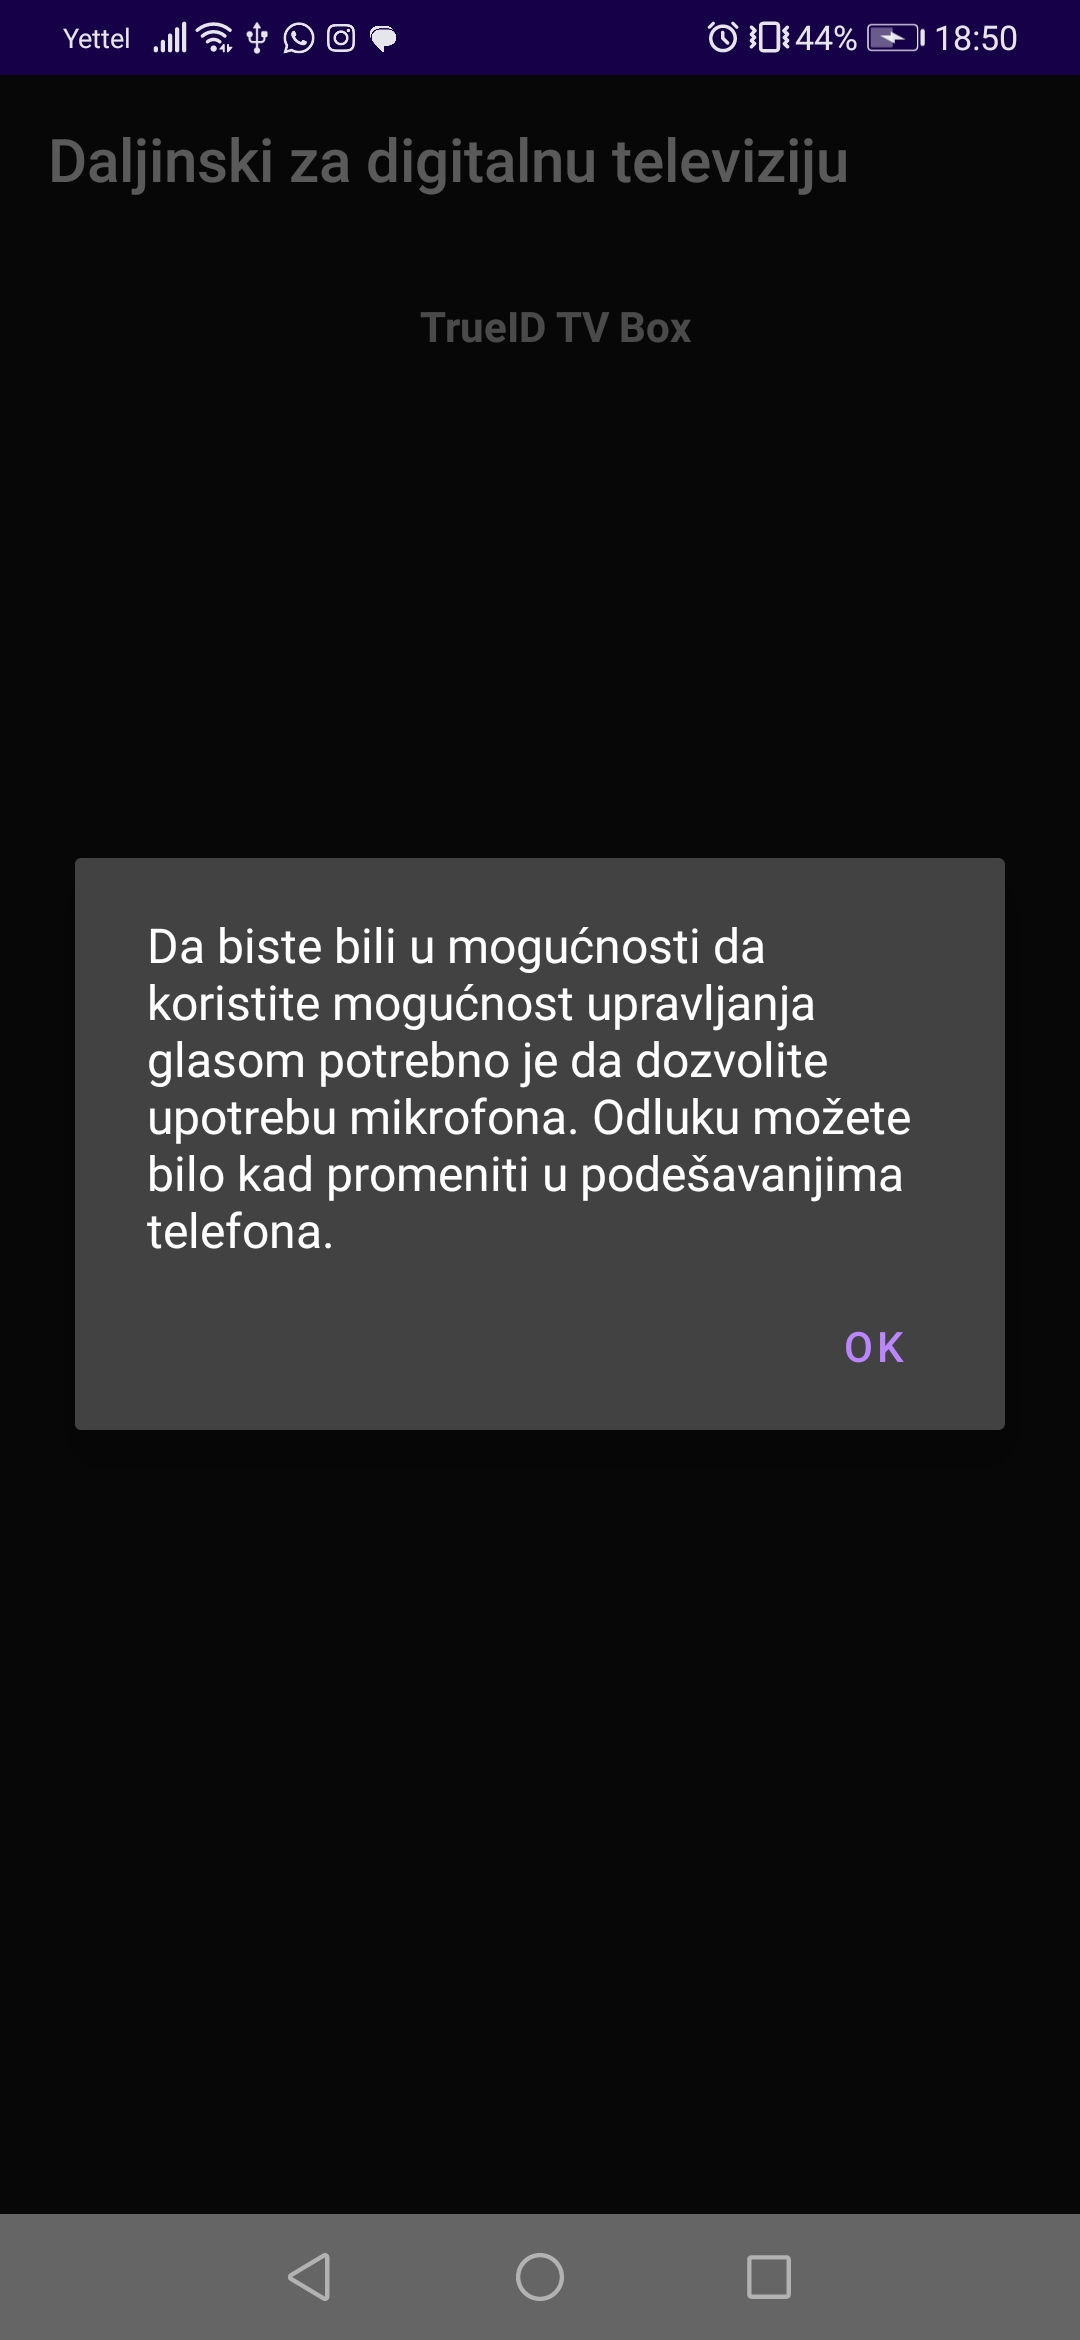
\includegraphics[width=9cm,height=9cm,keepaspectratio]{Implementacija/snimci_ekrana/1_obavestenje_za_dozvolu.jpg}
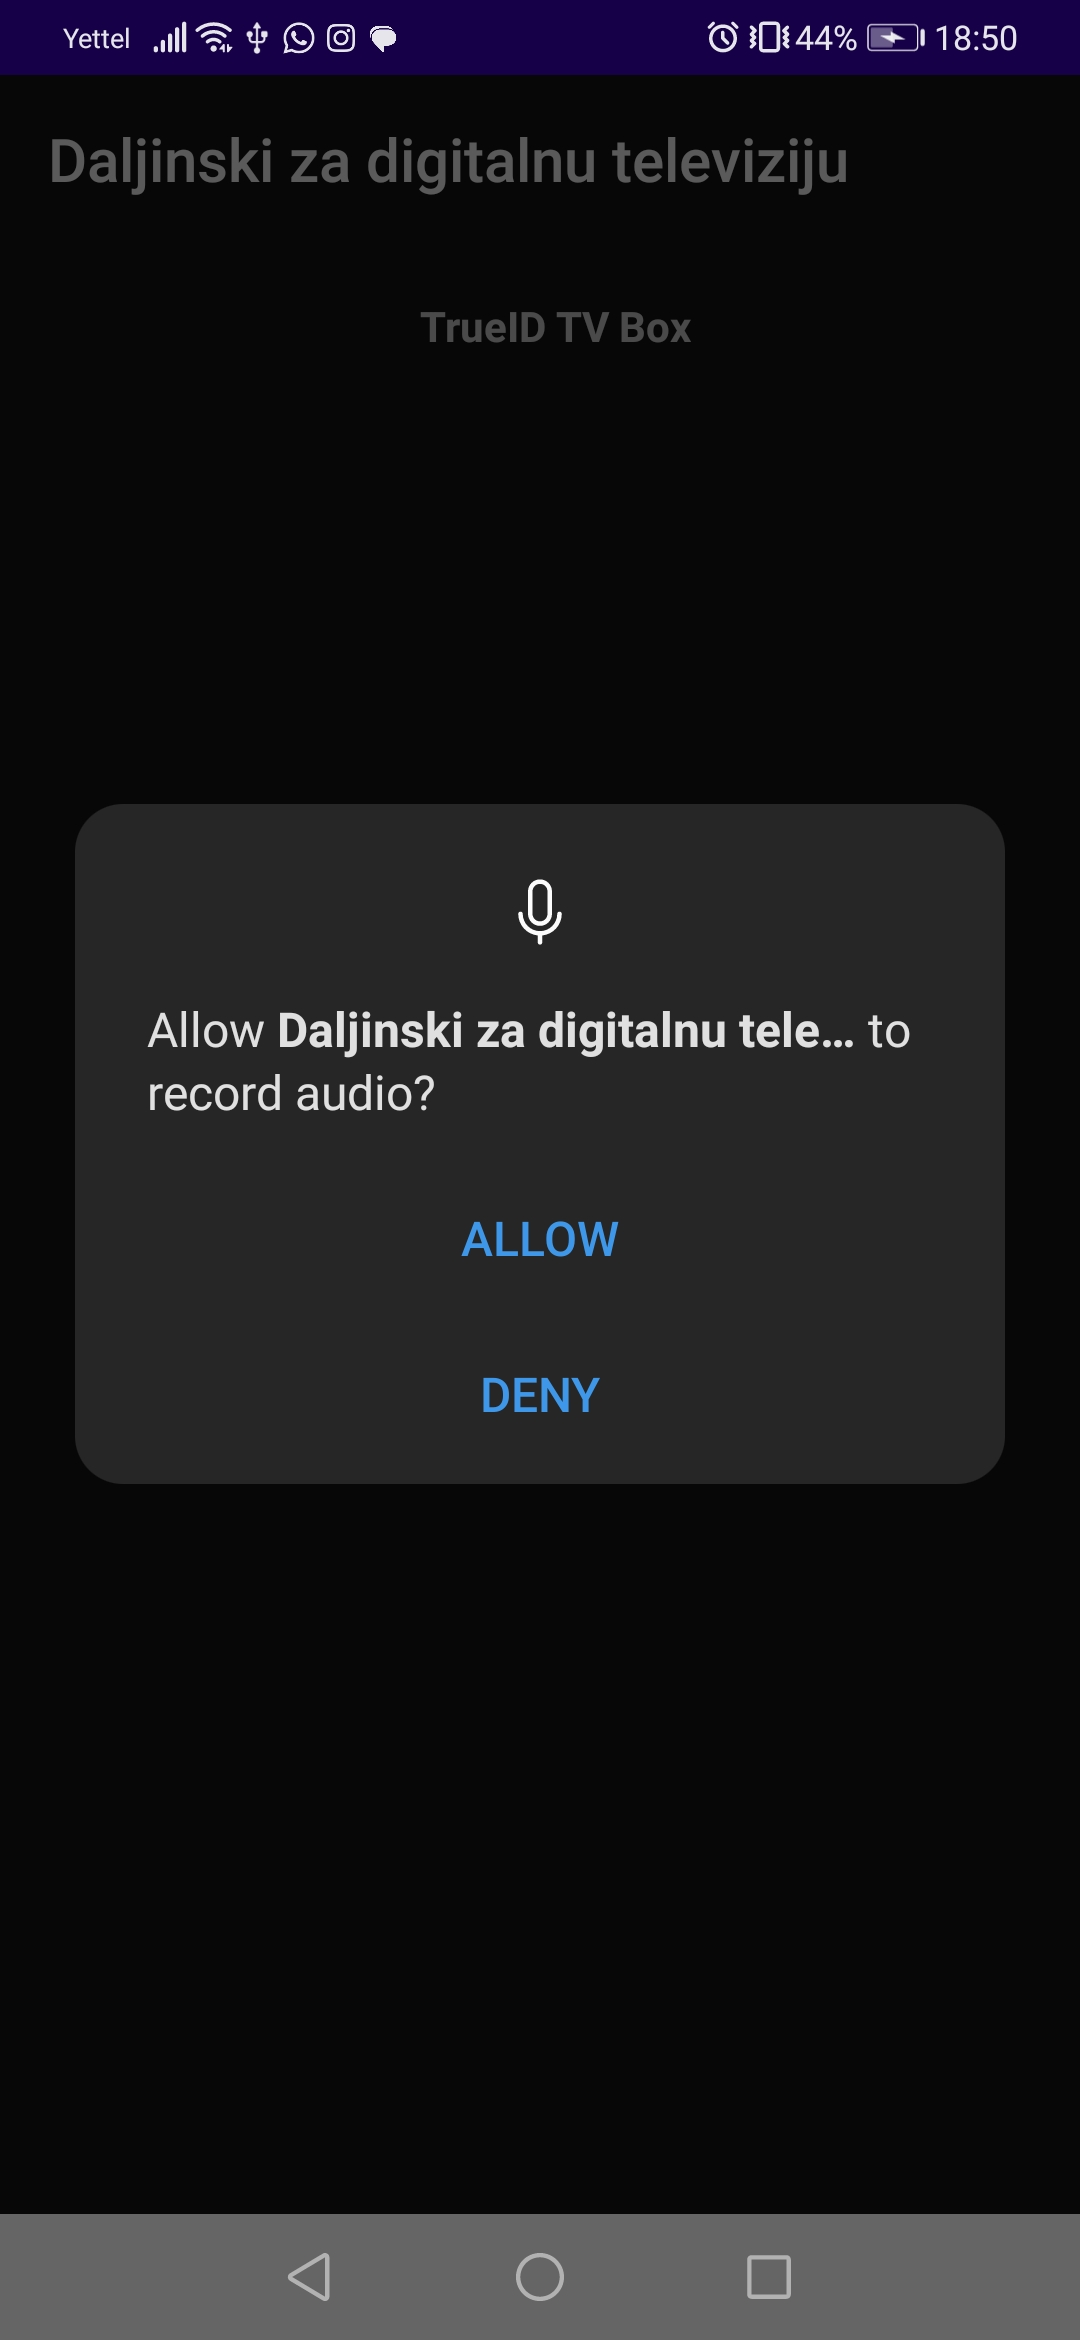
\includegraphics[width=9cm,height=9cm,keepaspectratio]{Implementacija/snimci_ekrana/2_sistemska_dozvola.jpg}
\caption{Snimci ekrana: A. obaveštenje o traženju dozvole, B prikaz sistemskog obaveštenja}
\end{figure}


% ----------------------------------------------------
\begin{figure}[h!]
\centering
\begin{minipage}{.5\textwidth}
  \centering
  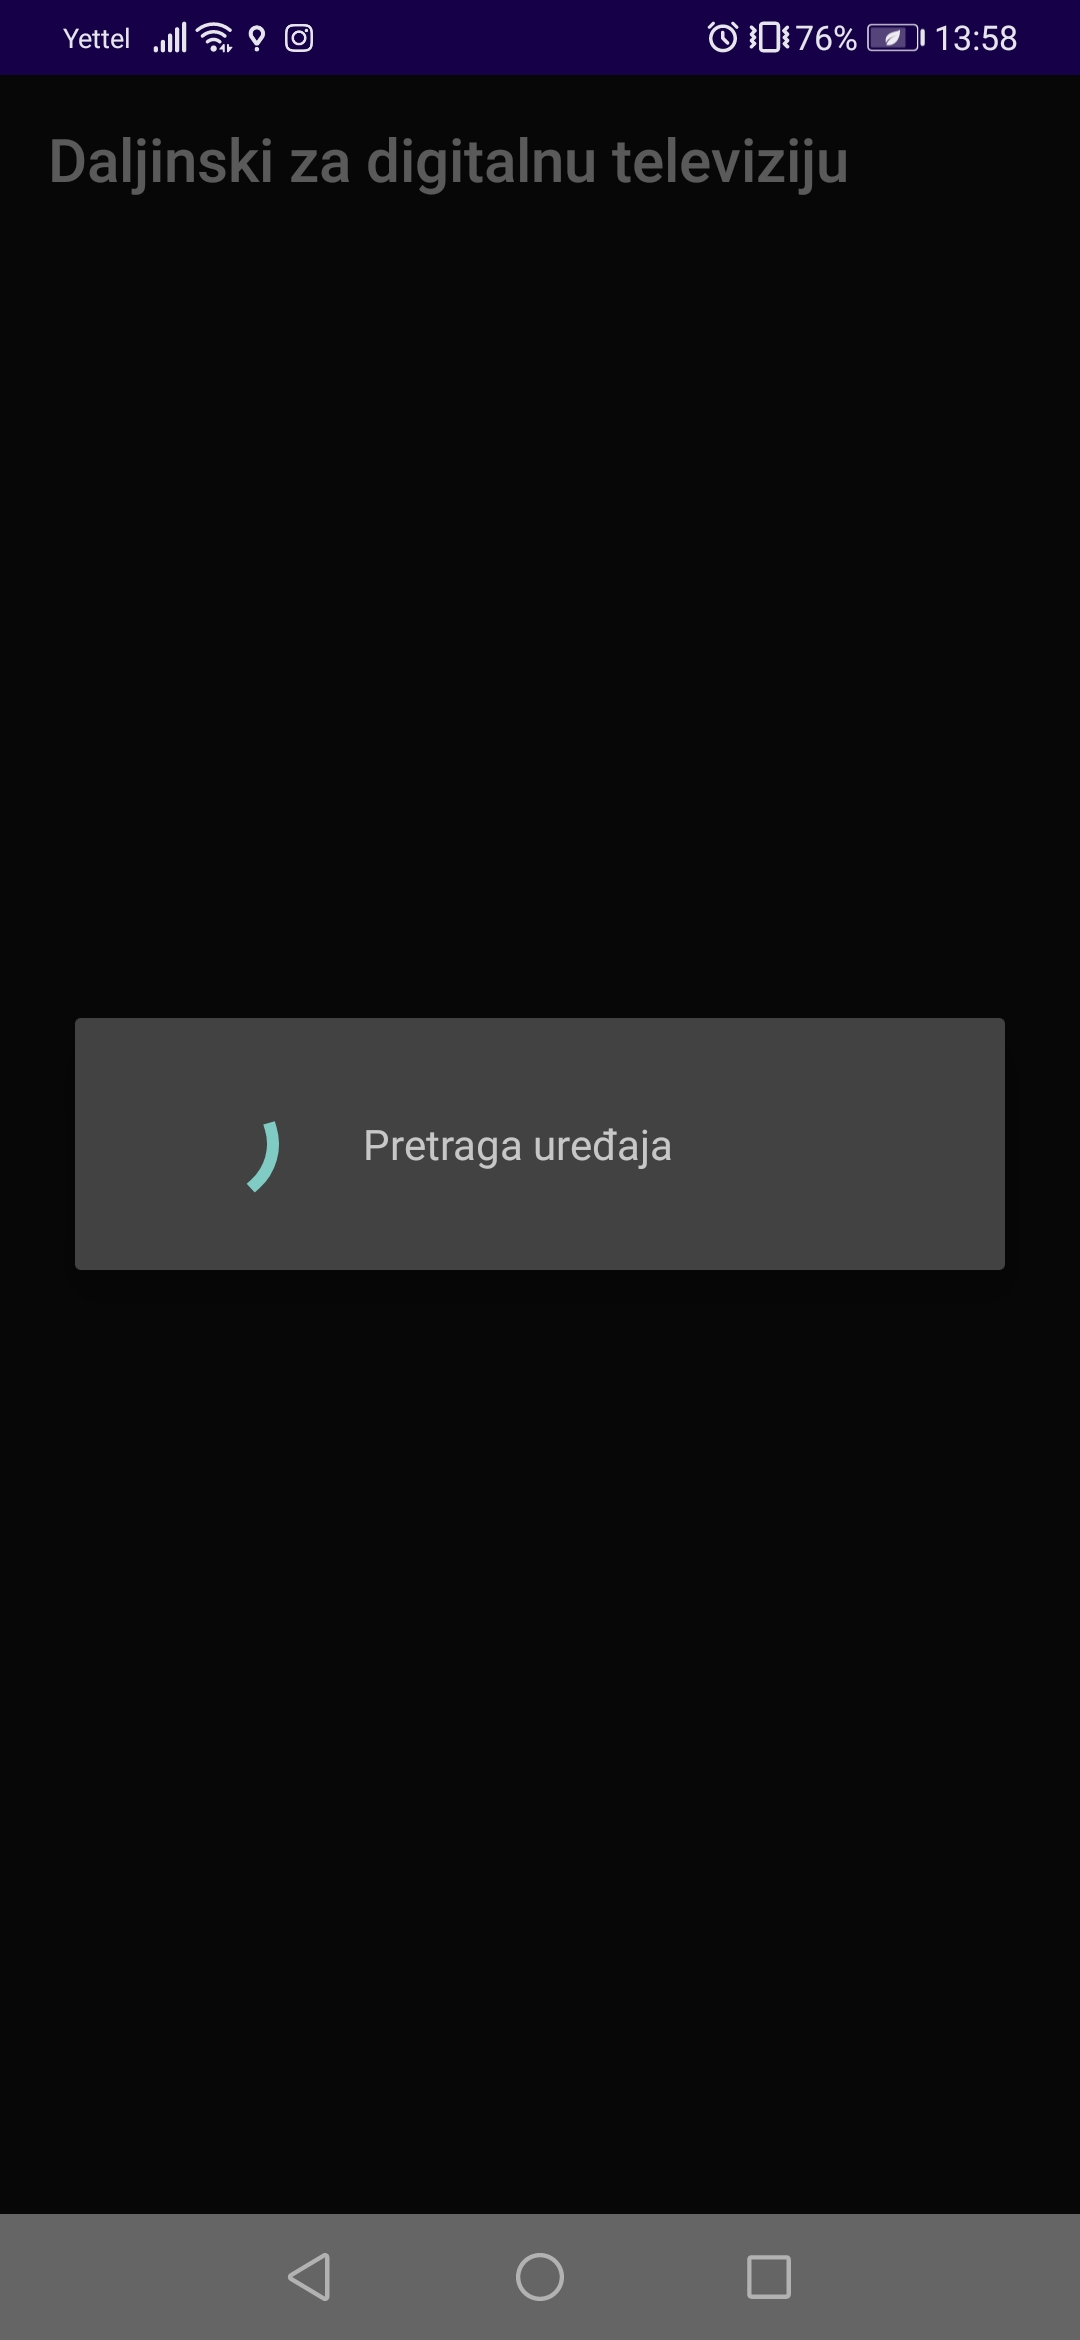
\includegraphics[width=9cm,height=9cm,keepaspectratio]{Implementacija/snimci_ekrana/3_pretraga_uredjaja.jpg}
  \caption{Snimak ekrana, pretraga uređaja}
   \label{fig:pretraga}
\end{minipage}%
\begin{minipage}{.5\textwidth}
   \centering
  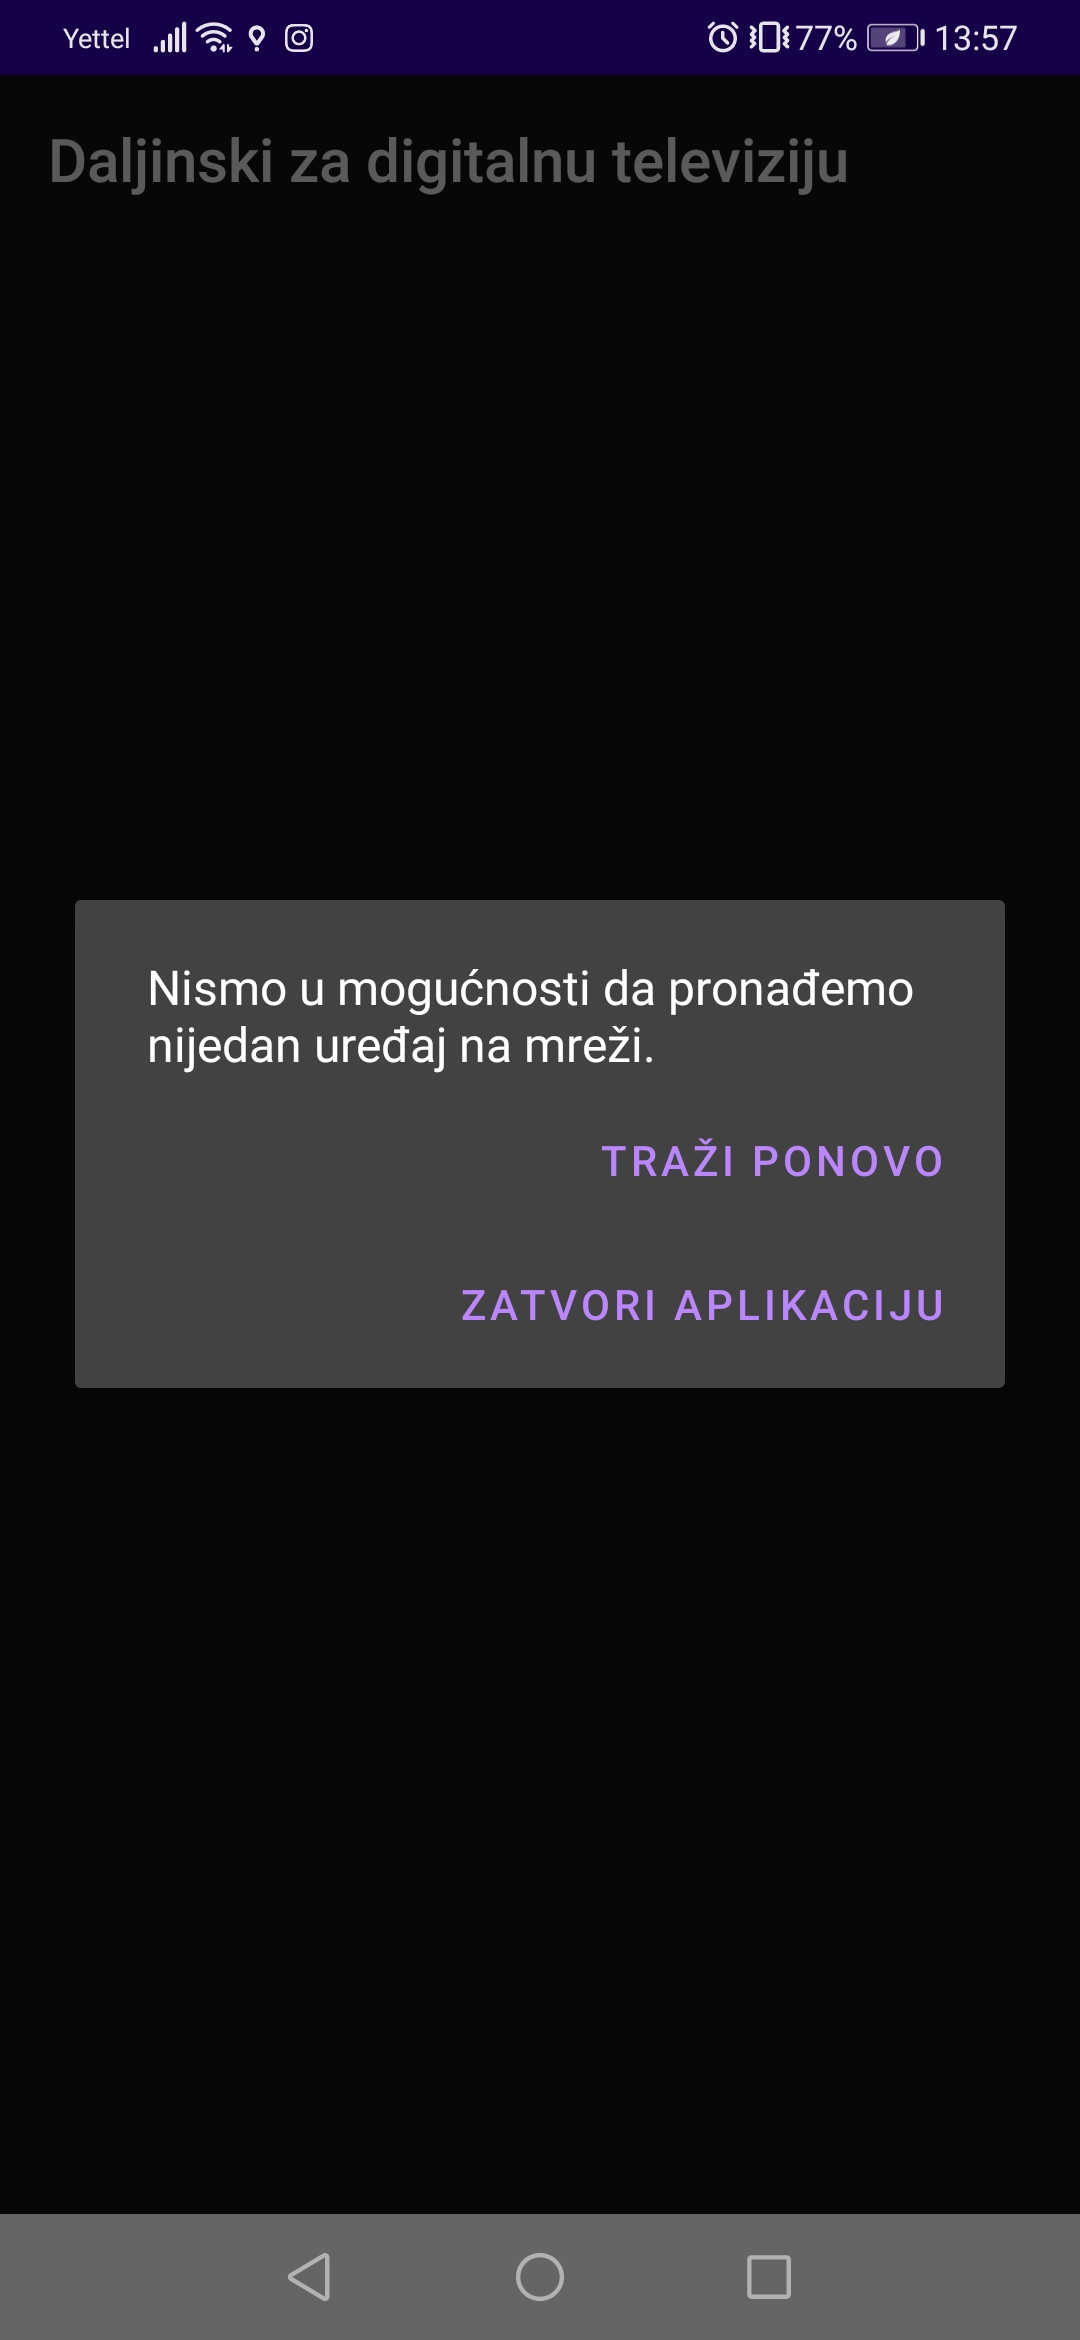
\includegraphics[width=9cm,height=9cm,keepaspectratio]{Implementacija/snimci_ekrana/4_uredjaji_nisu_pronadjeni.jpg}
  \caption{Snimak ekrana, nisu pronađeni uređaji}
   \label{fig:nema_uredjaja}
\end{minipage}
\end{figure}

% ----------------------------------------------------
\begin{figure}[h!]
\centering
\begin{minipage}{.5\textwidth}
 \centering
  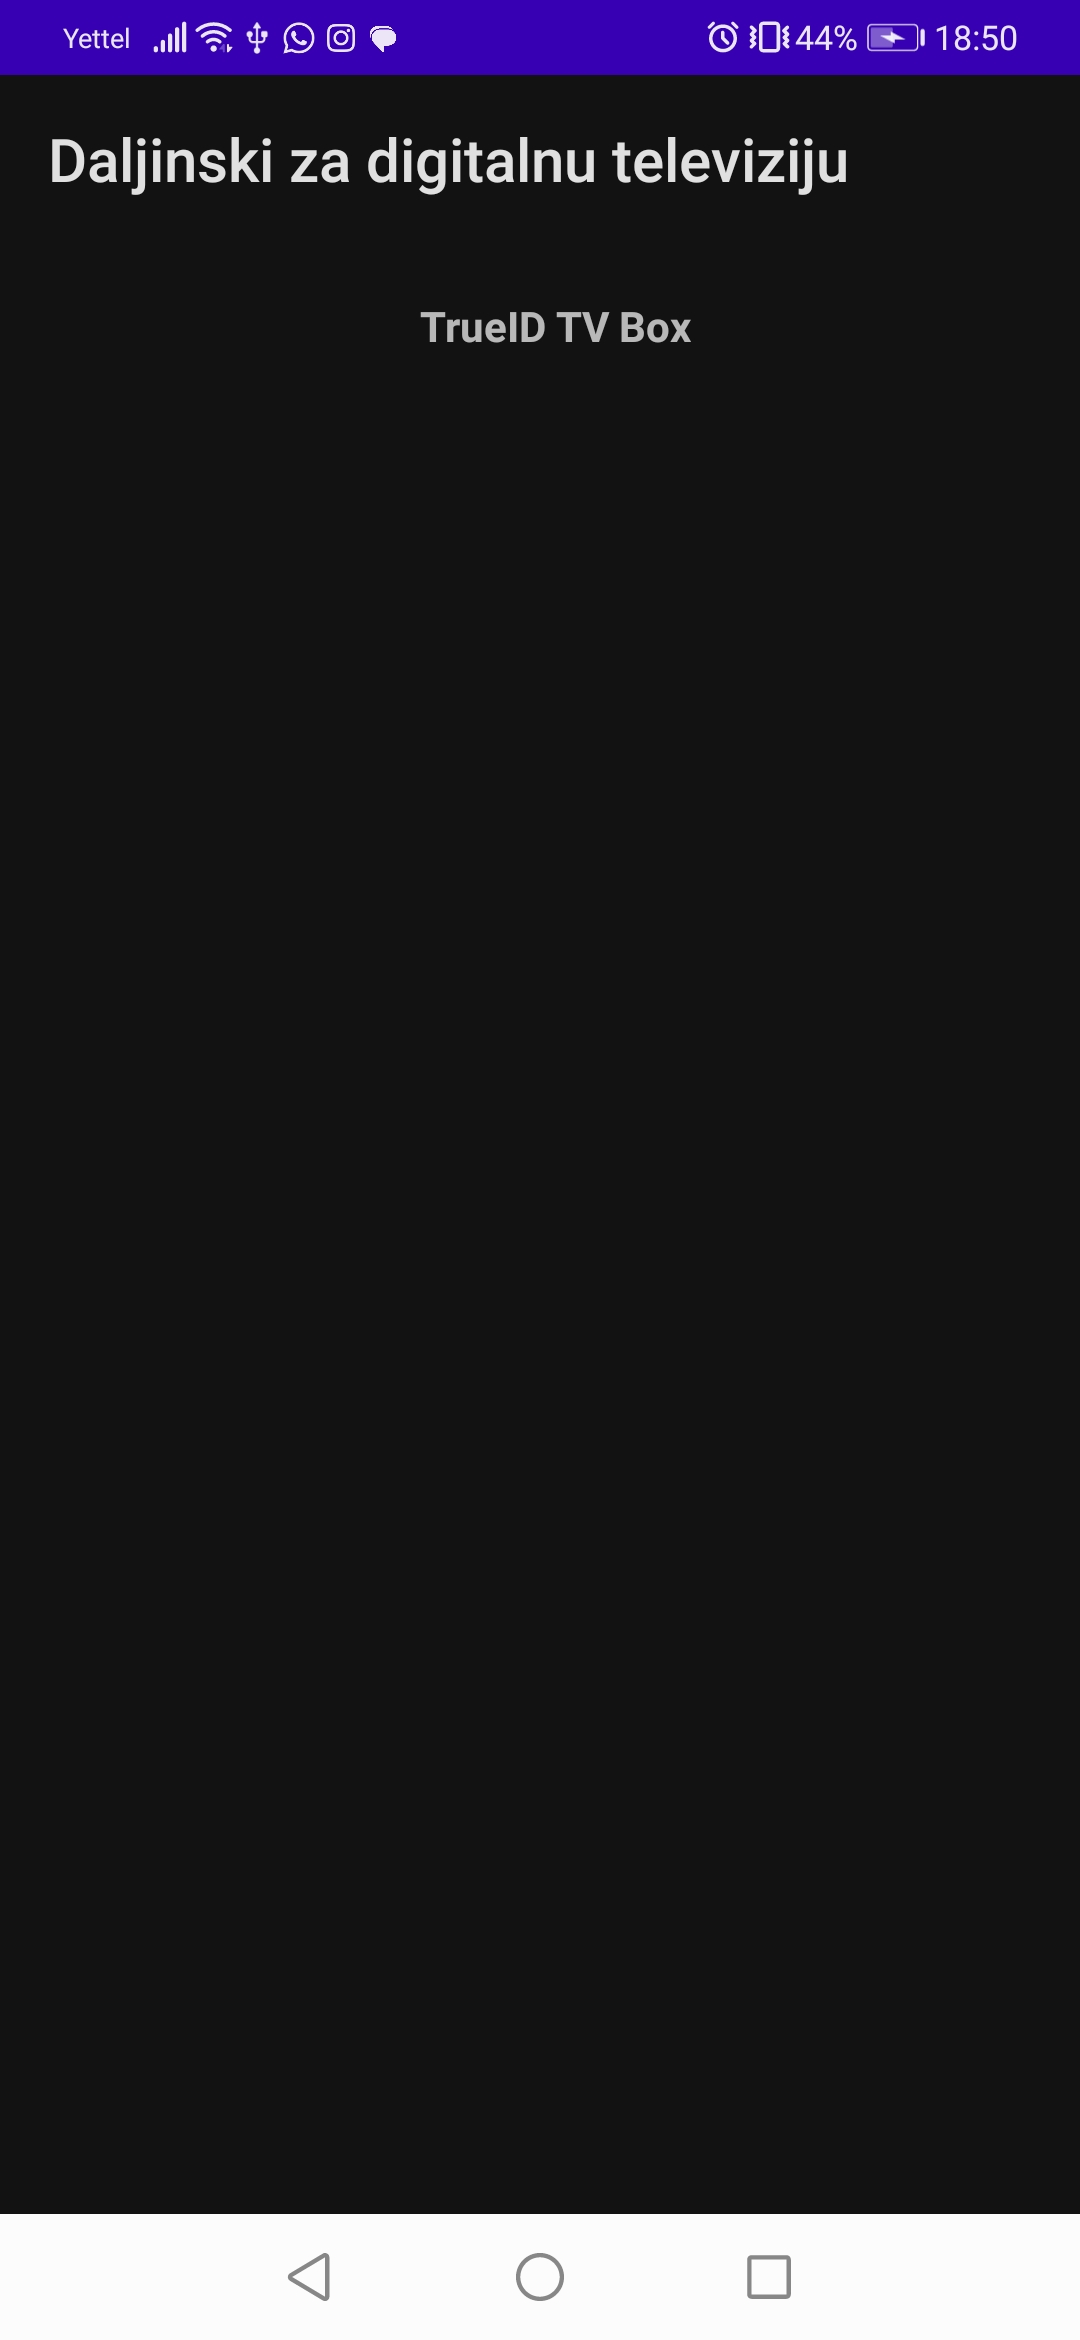
\includegraphics[width=9cm,height=9cm,keepaspectratio]{Implementacija/snimci_ekrana/5_pronadjeni_uredjaji.jpg}
  \caption{Snimak ekrana, pronađeni uređaji}
  \label{fig:pronadjeni_uredjaji}
\end{minipage}%
\begin{minipage}{.5\textwidth}
   \centering
  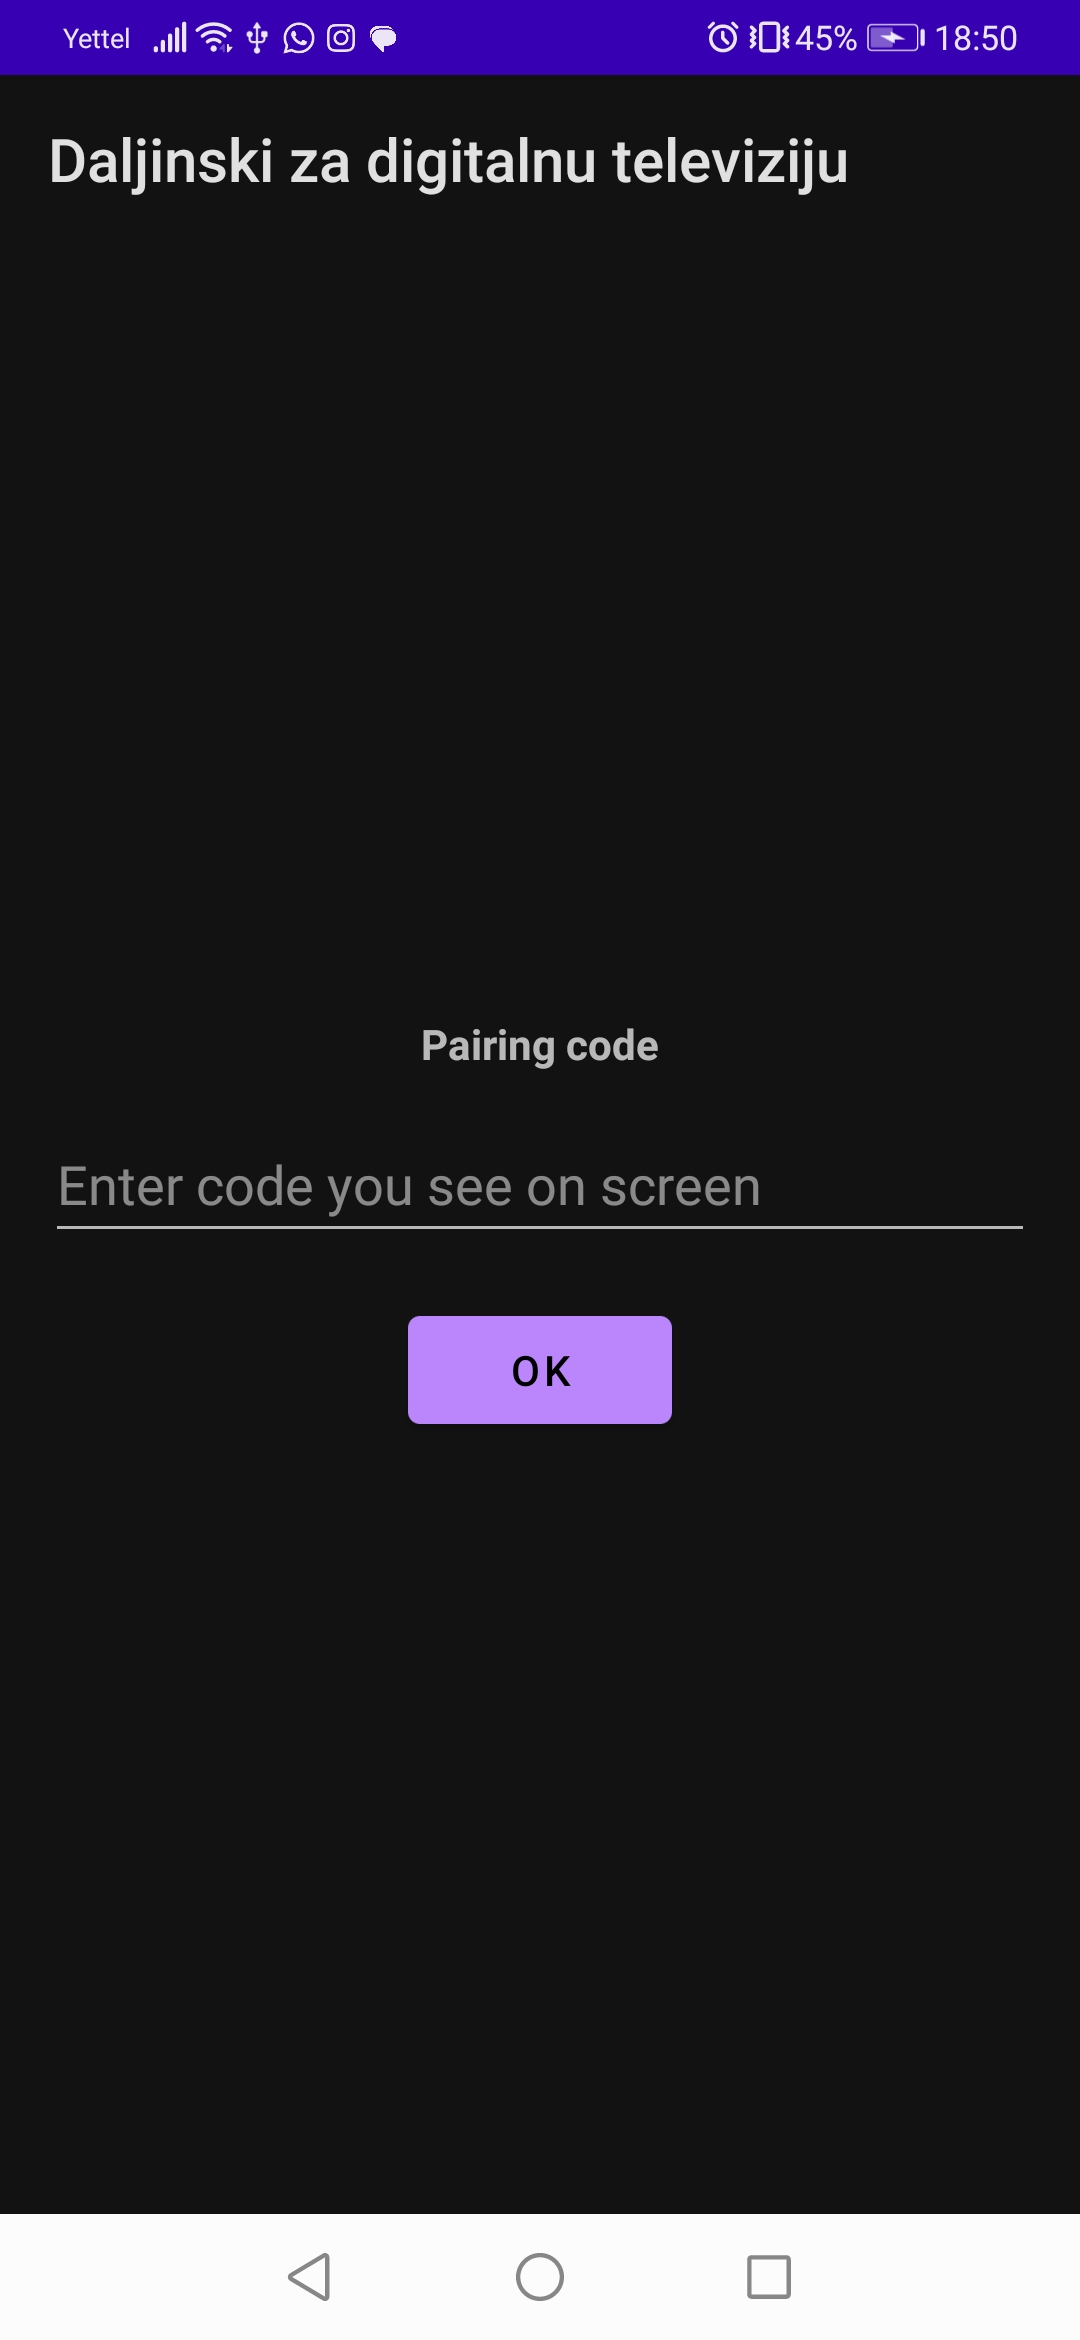
\includegraphics[width=9cm,height=9cm,keepaspectratio]{Implementacija/snimci_ekrana/6_uparivanje_sa_uredjajem.jpg}
  \caption{Snimak ekrana, polje za unos koda}
  \label{fig:polje_za_kod}
\end{minipage}
\end{figure}

% ----------------------------------------------------
\begin{figure}[h!]
\centering
\begin{minipage}{.6\textwidth}
 \centering
  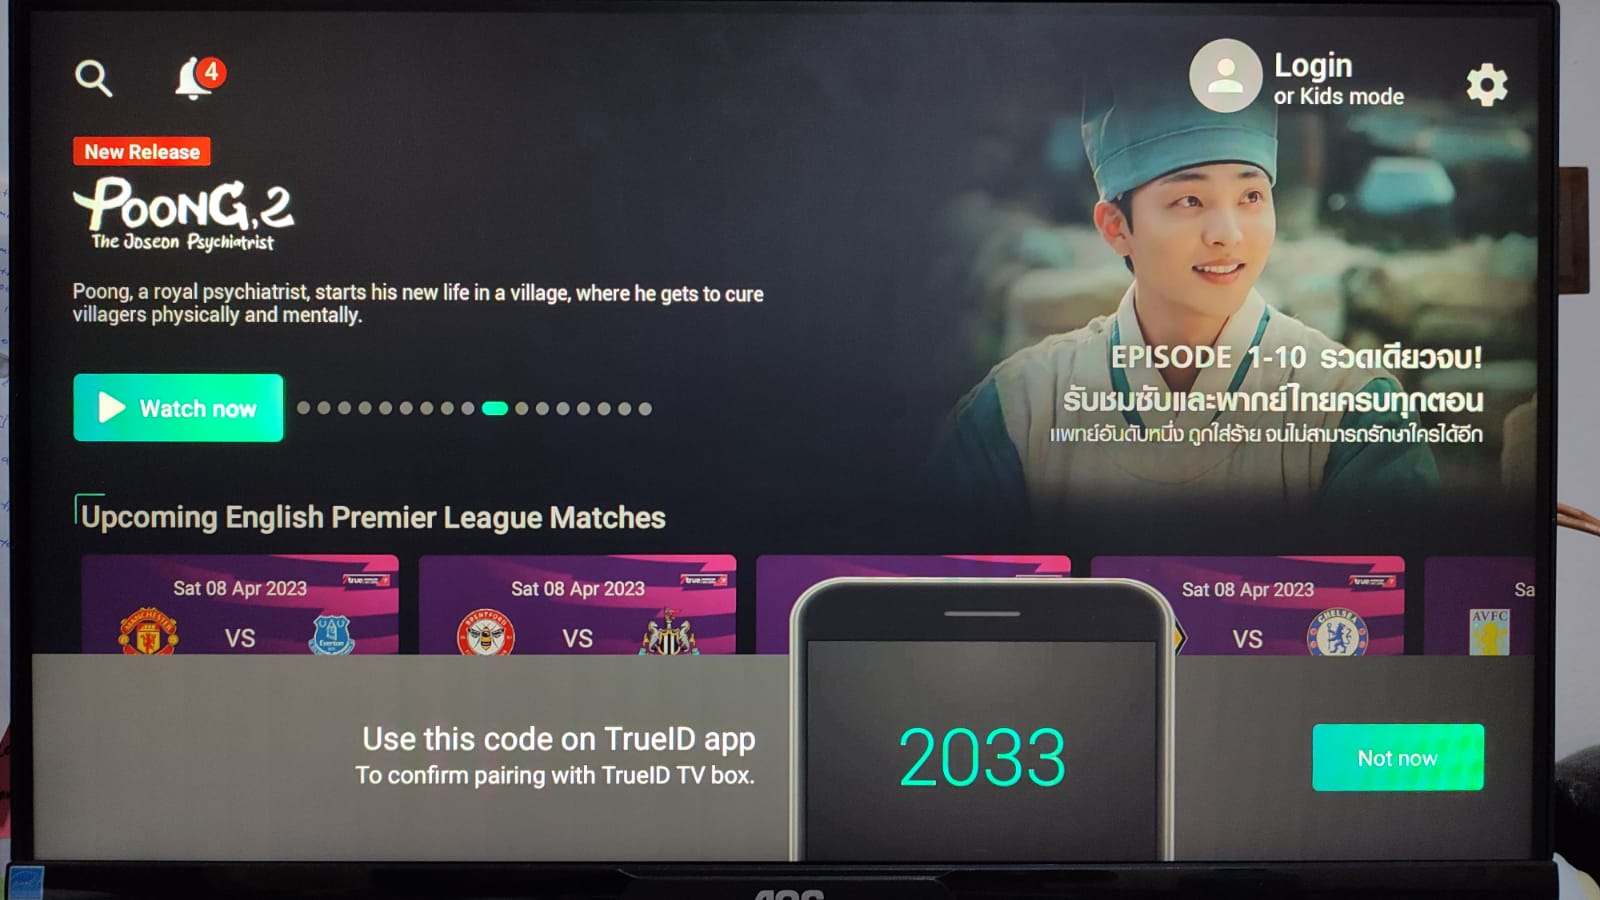
\includegraphics[width=9cm,height=9cm,keepaspectratio]{Implementacija/snimci_ekrana/8_kod_za_uparivanje_na_stb.jpg}
  \caption{Snimak ekrana, k\^{o}d za uparivanje na uređaju}
  \label{fig:kod_na_stb}
\end{minipage}%
\begin{minipage}{.4\textwidth}
   \centering
  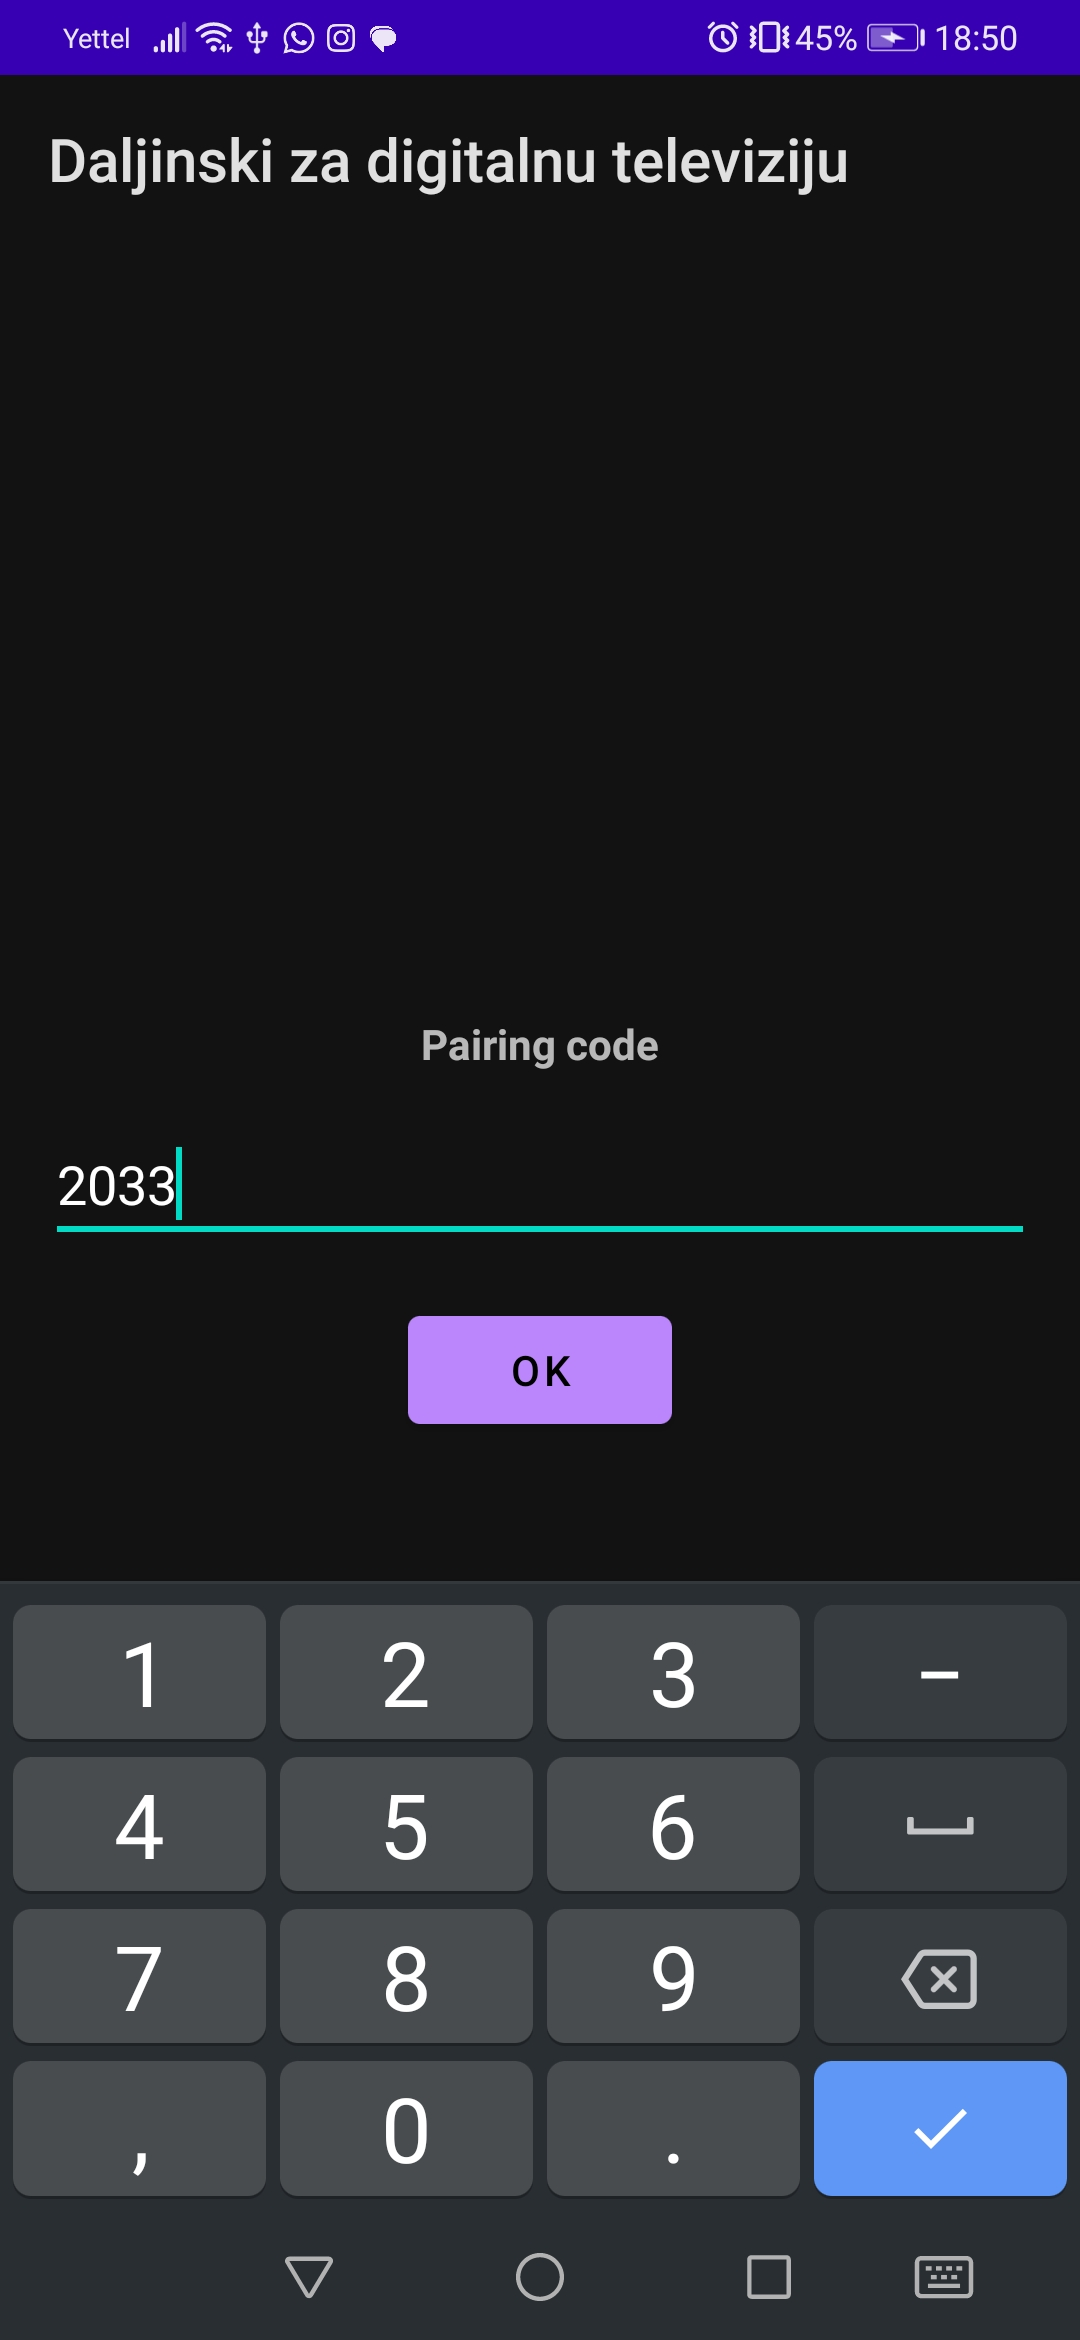
\includegraphics[width=9cm,height=9cm,keepaspectratio]{Implementacija/snimci_ekrana/7_unos_koda_za_uparivanje.jpg}
  \caption{Snimak ekrana, polje za unos koda}
   \label{fig:kod_na_mobilnom}
\end{minipage}
\end{figure}


Dalje korišćenje aplikacije je isto kao i korišćenje fizičkog daljinskog upravljača. Pri svakom pritisku dugmeta će korisnik osetiti blagu vibraciju što ujedno obaveštava i da je dugme pritisnuto. U slučaju kada nije data dozvola za korišćenje mikrofona nije moguće zadavati komande glasom i tada su dugmići za mikrofone onemogućeni i precrtani. U suprotnom korisnik može neometano da ih koristi.
\begin{description}
\item[Levo dugme] za mikrofon koje je tamnije boje koristi \textit{Google Cloud API}. Pri pritisku dugmeta na donjem delu ekrana pojaviće se poruka da je snimanje započeto i dugme će biti onemogućeno dokle god mikrofon sluša. Nakon pet sekundi prikazaće se poruka da je snimanje završeno, dugme će biti omogućeno i ukoliko je prepoznata komanda ona će se izvršiti.
\item[Desno dugme] koje je svetlije boje pokreće mikrofon generisan na standardni način koji obezbeđuje \textit{Google}. Pritiskom na dugme se pojavljuje polje generisano od strane \textit{Google}-a kao na slici \ref{fig:google_slusanje}. Izgled tog polja pri neuspešnom slušanju je prikazan na slici \ref{fig:google_neuspesno}, a pri uspešnom na slici \ref{fig:google_uspesno}. Pri uspešnom slušanju kao i u prethodnom slučaju izvršiće se zadata komanda.
\end{description}
Komande koje su podržane na ovaj način će biti izlistane u nastavku rada.  

\begin{figure}[h!]
  \centering
  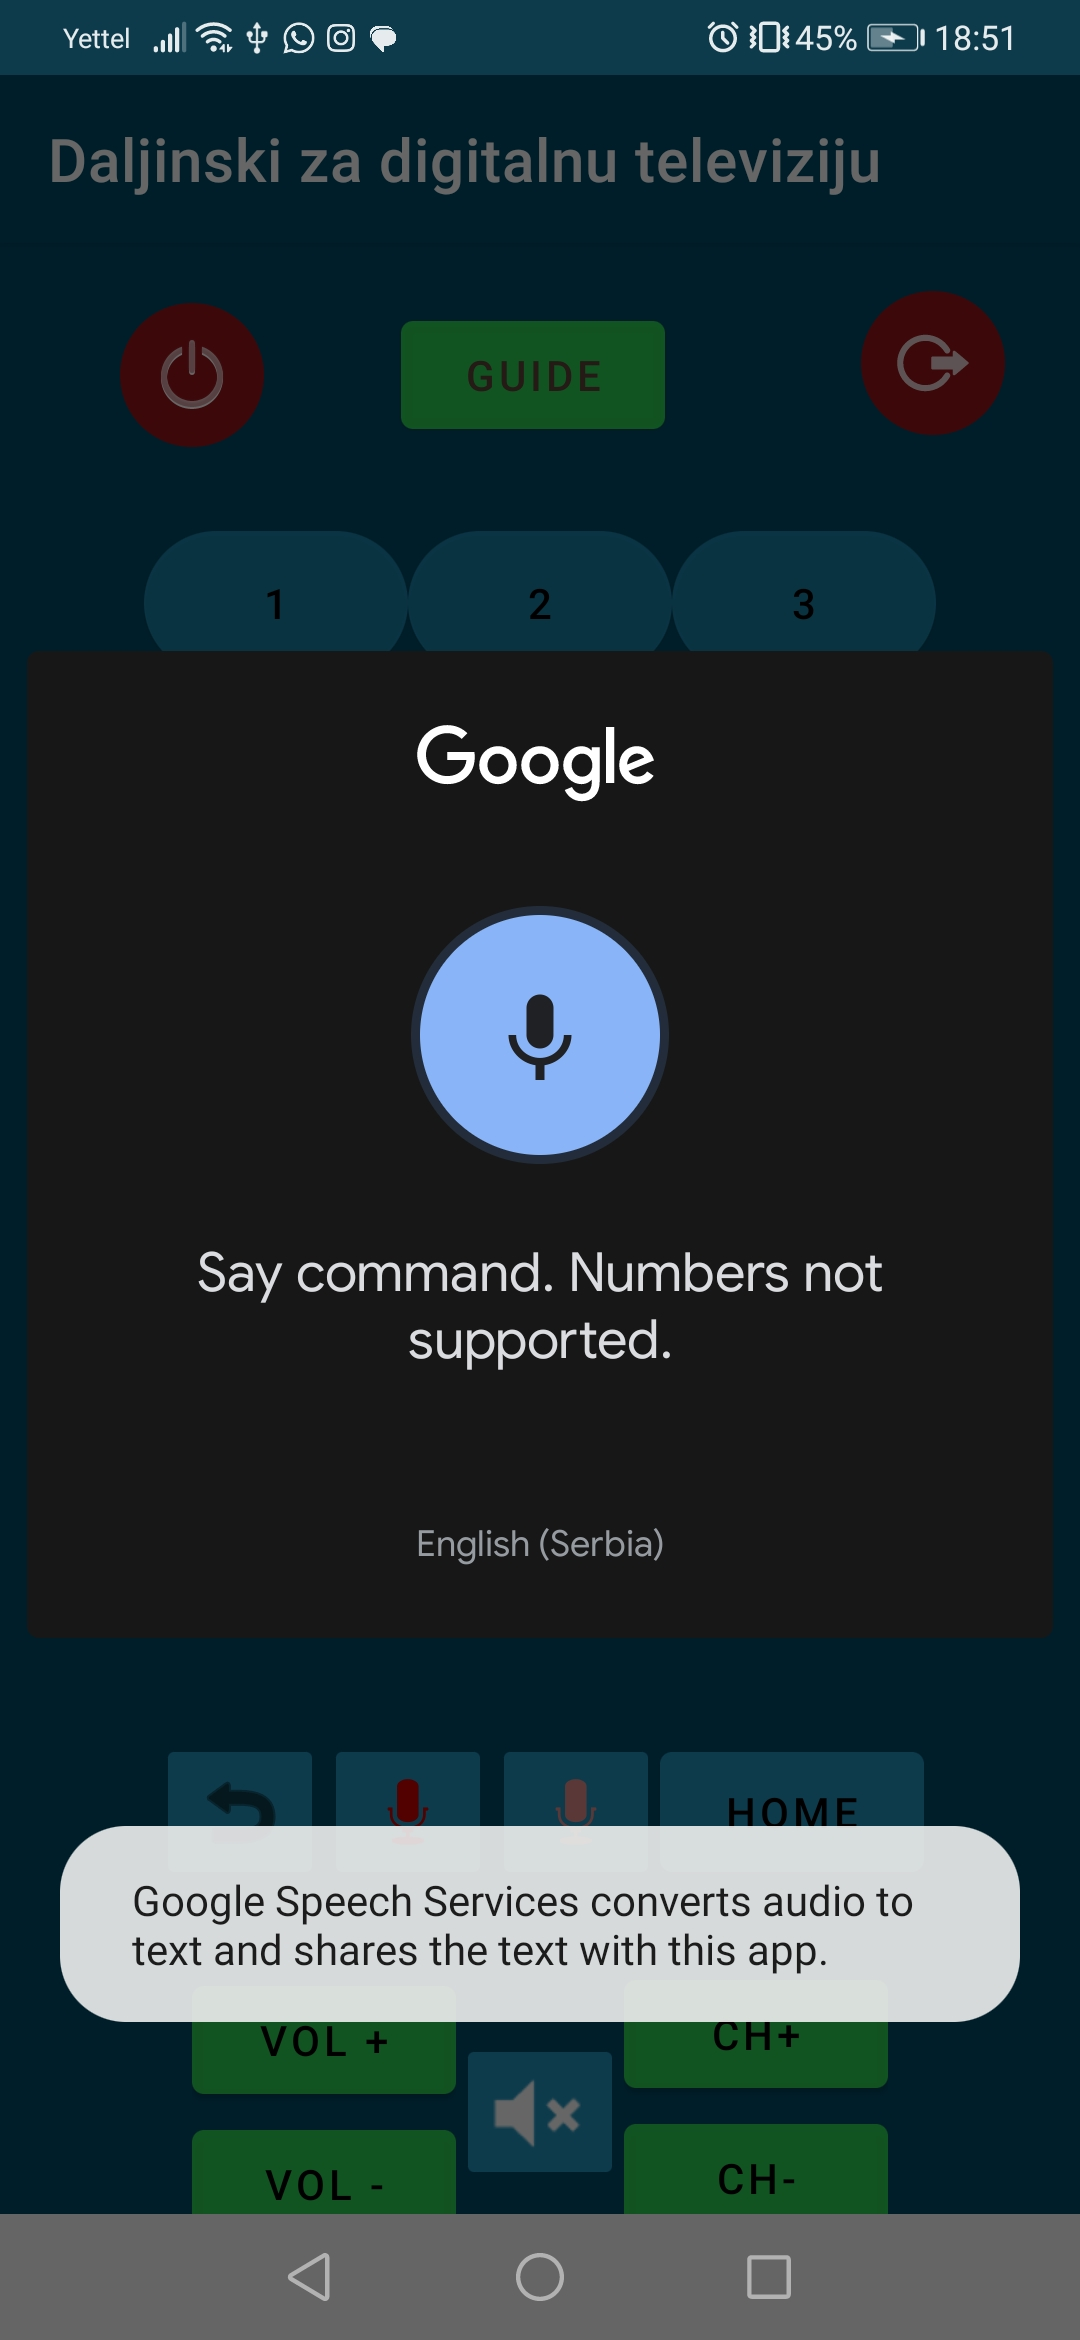
\includegraphics[width=9cm,height=9cm,keepaspectratio]{Implementacija/snimci_ekrana/10_obican_google_slusanje.jpg}
  \caption{Snimak ekrana, Google generisano polje za slušanje}
   \label{fig:google_slusanje}
\end{figure}


\begin{figure}[h!]
\centering
\begin{minipage}{.5\textwidth}
  \centering
  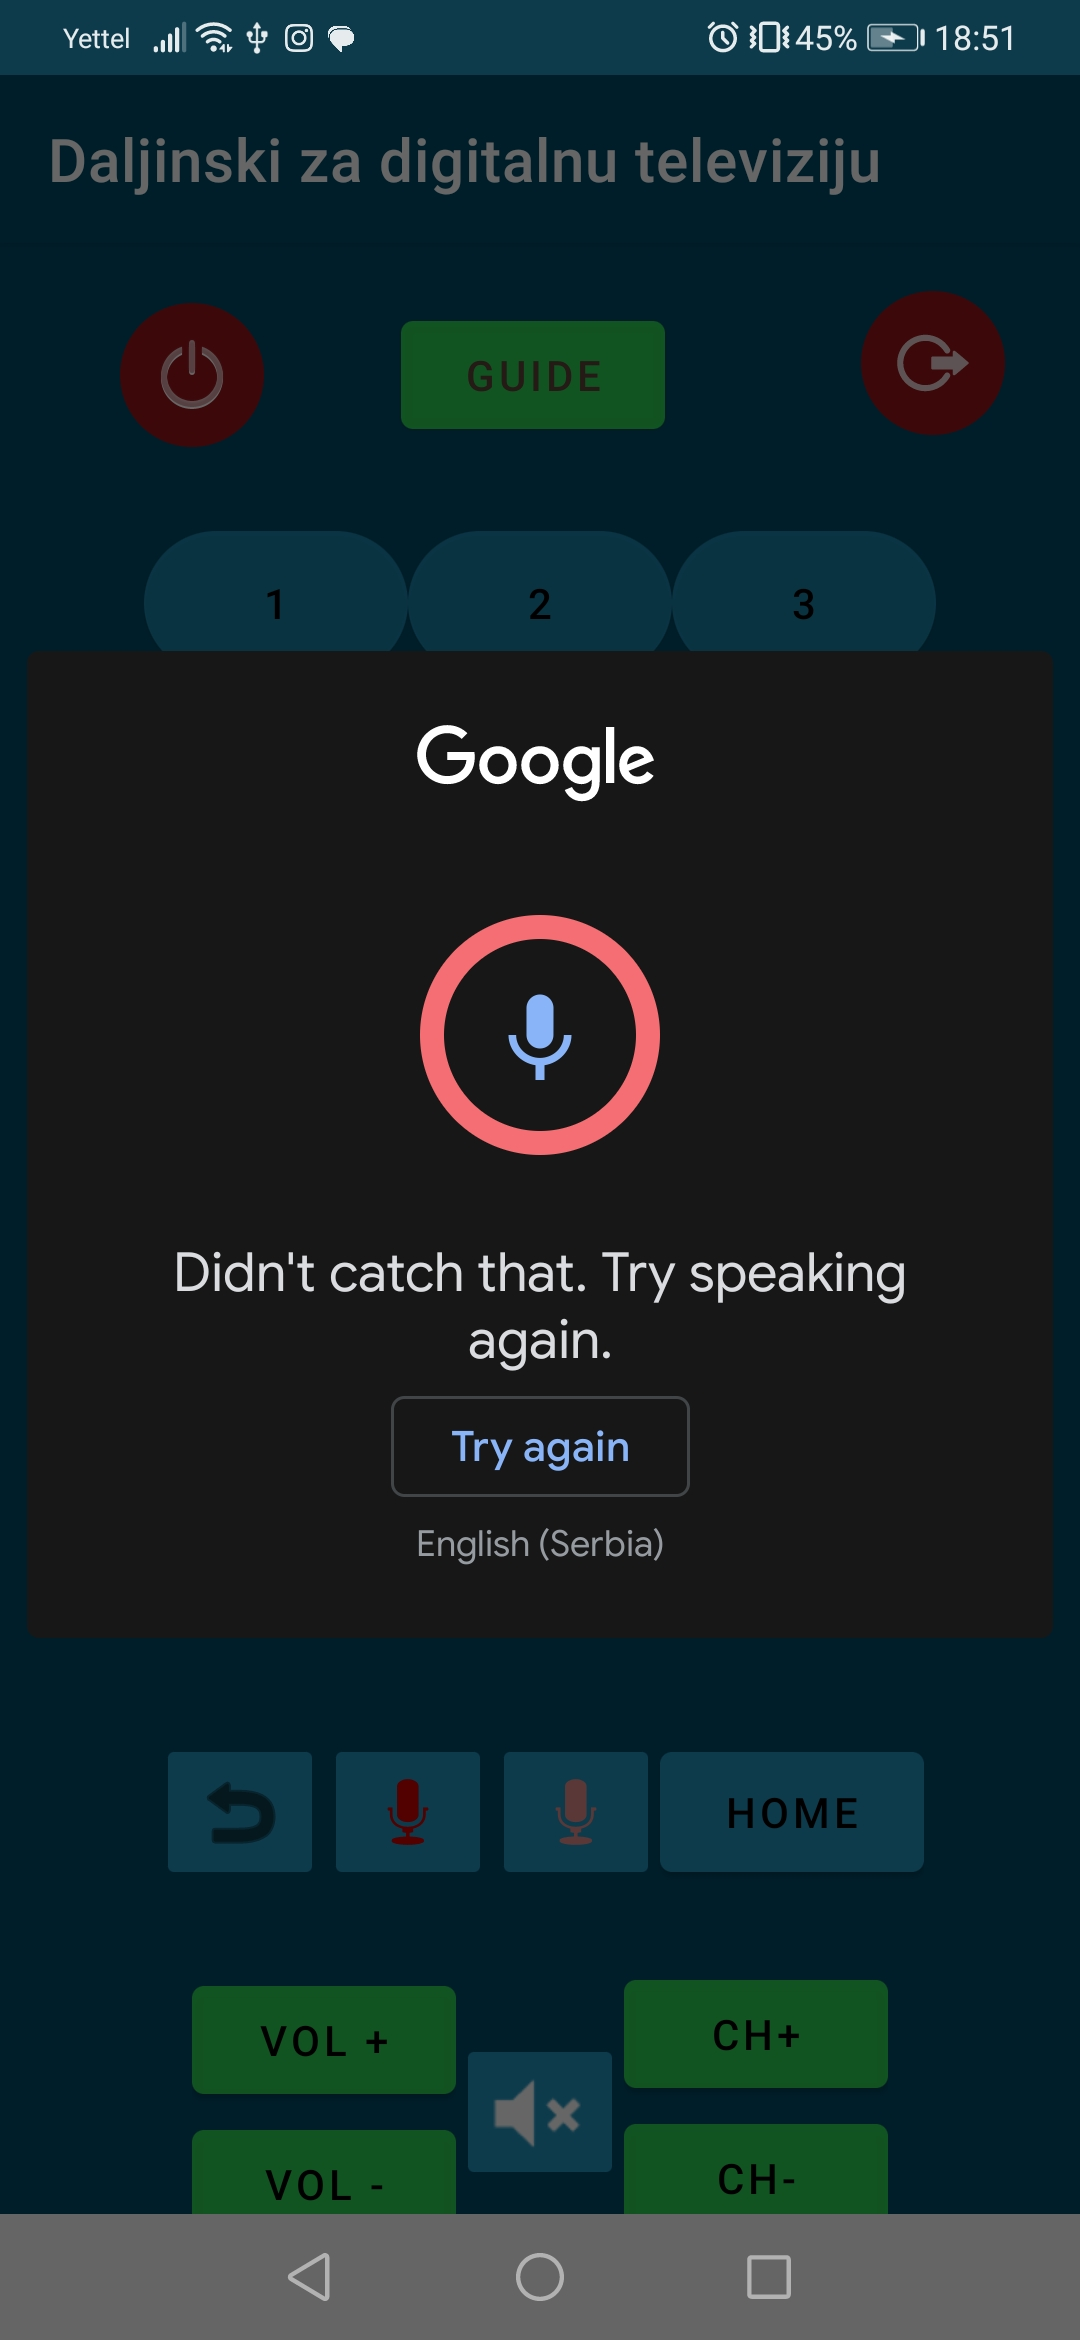
\includegraphics[width=9cm,height=9cm,keepaspectratio]{Implementacija/snimci_ekrana/11_obican_google_neuspesno.jpg}
  \caption{Snimak ekrana, Google generisano polje za slušanje prikaz neuspeha}
  \label{fig:google_neuspesno}
\end{minipage}%
\begin{minipage}{.5\textwidth}
  \centering
  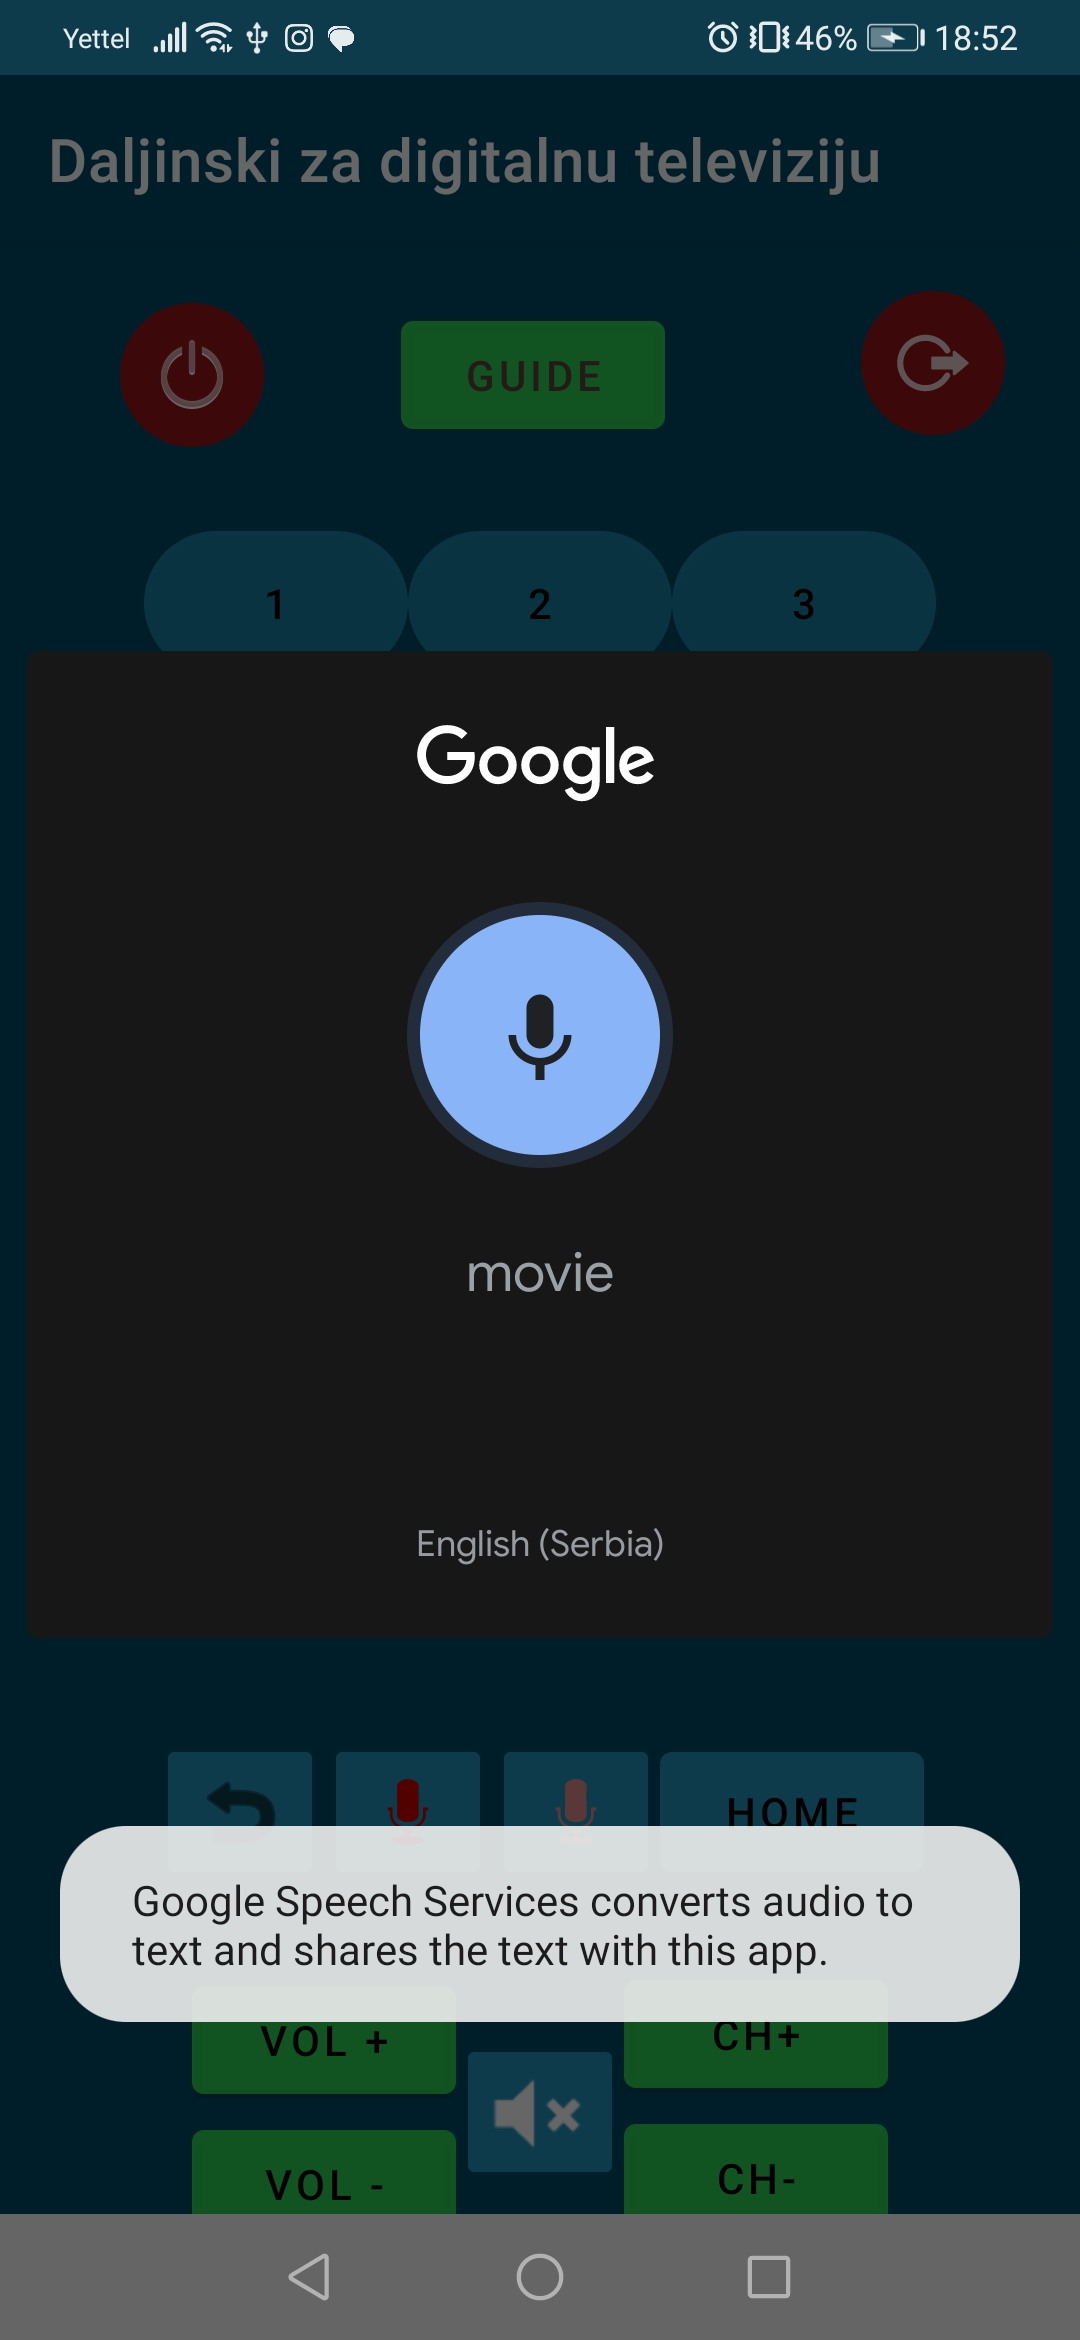
\includegraphics[width=9cm,height=9cm,keepaspectratio]{Implementacija/snimci_ekrana/11_obican_google_uspesno.jpg}
  \caption{Snimak ekrana, Google generisano polje za slušanje prikaz uspeha}
   \label{fig:google_uspesno}
\end{minipage}
\end{figure}

Ukoliko korisnik želi da prekine konekciju sa uređajem dovoljno je da pritisne dugme za otkazivanje konekcije koje ga vraća na početni ekran aplikacije. Tada će ponovo biti ivršena pretraga i izlistani pronađeni uređaji. Izlazak iz aplikacije bez prekida konekcije omogućava da korisnik ostane povezan sa uređajem i da pri sledećem pokretanju aplikacije odmah može da koristi sve funkcionalnosti bez ponovnog povezivanja.

\begin{figure}[h!]
  \centering
  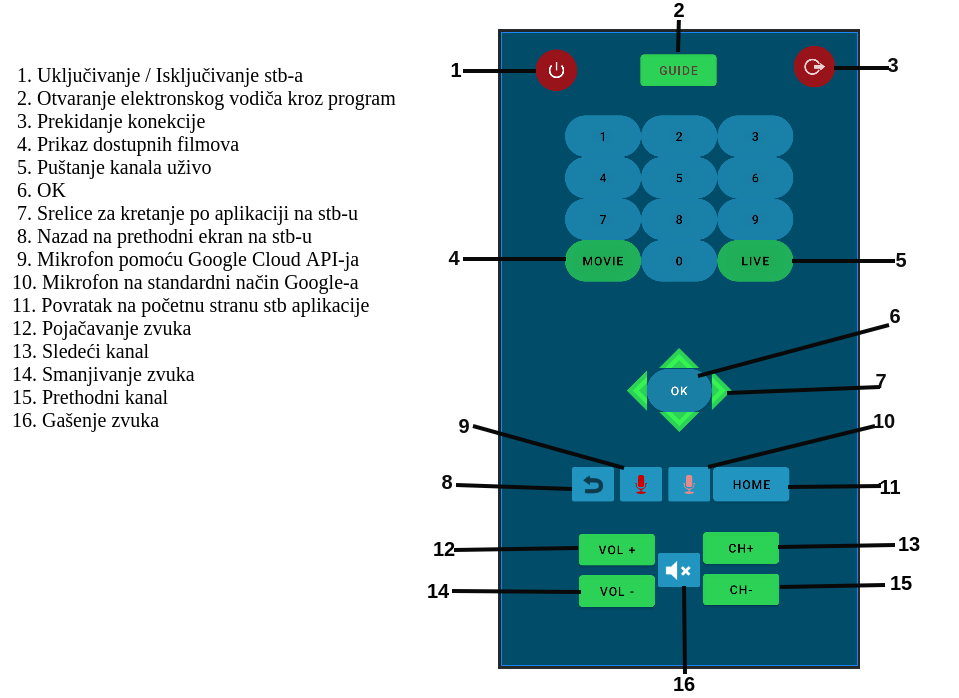
\includegraphics[width=\textwidth]{Implementacija/snimci_ekrana/komande_sa_opisom.png}
  \caption{Snimak ekrana, opis komandi}
   \label{fig:opis_komandi}
\end{figure}

\end{document}